\documentclass[12pt,dvipdfmx]{beamer}
%\usepackage{amsmath,amssymb,latexsym}
%\usepackage{stmaryrd}
%\usepackage{textcomp}
\usepackage{pgfpages}
\usepackage{graphicx}
\DeclareGraphicsExtensions{.eps}
\usepackage{listings,jlisting}
\usepackage{fancybox}
\usepackage{hyperref}

%%%%%%%%%%%%%%%%%%%%%%%%%%%
%%% \ifeng \ifjp
%%%%%%%%%%%%%%%%%%%%%%%%%%%
\newif\ifen
\entrue
%\enfalse
\newif\ifja
%\jatrue
\jafalse

%%%%%%%%%%%%%%%%%%%%%%%%%%%
%%% themes
%%%%%%%%%%%%%%%%%%%%%%%%%%%
\usetheme{Boadilla}
%% no navigation bar
% default boxes Bergen Boadilla Madrid Pittsburgh Rochester
%% tree-like navigation bar
% Antibes JuanLesPins Montpellier
%% toc sidebar
% Berkeley PaloAlto Goettingen Marburg Hannover Berlin Ilmenau Dresden Darmstadt Frankfurt Singapore Szeged
%% Section and Subsection Tables
% Copenhagen Luebeck Malmoe Warsaw

%%%%%%%%%%%%%%%%%%%%%%%%%%%
%%% innerthemes
%%%%%%%%%%%%%%%%%%%%%%%%%%%
% \useinnertheme{circles}       % default circles rectangles rounded inmargin

%%%%%%%%%%%%%%%%%%%%%%%%%%%
%%% outerthemes
%%%%%%%%%%%%%%%%%%%%%%%%%%%
% outertheme
% \useoutertheme{default}       % default infolines miniframes smoothbars sidebar sprit shadow tree smoothtree


%%%%%%%%%%%%%%%%%%%%%%%%%%%
%%% colorthemes
%%%%%%%%%%%%%%%%%%%%%%%%%%%
\usecolortheme{seahorse}
%% special purpose
% default structure sidebartab 
%% complete 
% albatross beetle crane dove fly seagull 
%% inner
% lily orchid rose
%% outer
% whale seahorse dolphin

%%%%%%%%%%%%%%%%%%%%%%%%%%%
%%% fontthemes
%%%%%%%%%%%%%%%%%%%%%%%%%%%
\usefonttheme{serif}  
% default professionalfonts serif structurebold structureitalicserif structuresmallcapsserif

%%%%%%%%%%%%%%%%%%%%%%%%%%%
%%% generally useful beamer settings
%%%%%%%%%%%%%%%%%%%%%%%%%%%
% 
\AtBeginDvi{\special{pdf:tounicode EUC-UCS2}}
% do not show navigation
\setbeamertemplate{navigation symbols}{}
% show page numbers
\setbeamertemplate{footline}[frame number]


%%%%%%%%%%%%%%%%%%%%%%%%%%%
%%% define some colors for convenience
%%%%%%%%%%%%%%%%%%%%%%%%%%%

\newcommand{\mido}[1]{{\color{brown}#1}}
\newcommand{\mura}[1]{{\color{purple}#1}}
\newcommand{\ore}[1]{{\color{orange}#1}}
\newcommand{\ao}[1]{{\color{blue}#1}}
\newcommand{\aka}[1]{{\color{red}#1}}
\newcommand{\hai}[1]{{\color{gray}#1}}

\setbeamercolor{ex}{bg=cyan!20!white}

%%%%%%%%%%%%%%%%%%%%%%%%%%%
%%% how to typset code
%%%%%%%%%%%%%%%%%%%%%%%%%%%

\lstset{language = C,
numbers = left,
numberstyle = {\tiny \emph},
numbersep = 10pt,
breaklines = true,
breakindent = 40pt,
frame = tlRB,
frameround = ffft,
framesep = 3pt,
rulesep = 1pt,
rulecolor = {\color{blue}},
rulesepcolor = {\color{blue}},
flexiblecolumns = true,
keepspaces = true,
basicstyle = \ttfamily\scriptsize,
identifierstyle = ,
commentstyle = ,
stringstyle = ,
showstringspaces = false,
tabsize = 4,
escapechar=\@,
}

\ifja
\title{プログラミング言語 (5) \\ 言語処理系実装の基本}
\fi
\ifen
  \title{Programming Language (5) \\
    Basics of Programming Language Implementation}
\fi
\institute{}
\author{田浦}
\date{}

\AtBeginSection[] % Do nothing for \section*
{
\begin{frame}
\frametitle{Contents}
\tableofcontents[currentsection]
\end{frame}
}

\AtBeginSubsection[] % Do nothing for \section*
{
\begin{frame}
\frametitle{Contents}
\tableofcontents[currentsection,currentsubsection]
\end{frame}
}

\begin{document}
\maketitle

%%%%%%%%%%%%%%%%%%%%%%%%%%%%%%%%%% 
\begin{frame}
\ifja
\frametitle{目次}
\fi
\ifen
\frametitle{Contents}
\fi
\tableofcontents
\end{frame}

%%%%%%%%%%%%%%%%%%%%%%%%%%%%%%%%%%
\ifja
\section{はじめに}
\fi
\ifen
\section{Introduction}
\fi
%%%%%%%%%%%%%%%%%%%%%%%%%%%%%%%%%%

%%%%%%%%%%%%%%%%%%%%%%%%%%%%%%%%%% 
\ifja
\begin{frame}
\frametitle{言語処理系実装の形態}
\begin{itemize}
\item \ao{インタプリタ:} プログラムを解釈実行(プログラムと入力から出力を直接計算)
\item \ao{トランスレータ:} プログラムを別の言語(例: C)に翻訳
  \begin{itemize}
  \item 例: OpenMP (Cの並列拡張) を C (+ Pthreads) に翻訳
  \end{itemize}
\item \ao{コンパイラ:} プログラムを機械語に翻訳
\end{itemize}
\end{frame}
\fi

\ifen
\begin{frame}
\frametitle{Two basic forms of language implementation}
\begin{itemize}
\item \ao{interpreter:} interprets and executes programs
  (takes a program and an input; and computes the output)
\item \ao{compiler:} translates programs into \ao{a machine (assembly) code},
  that can directly execute by the processor
  \begin{itemize}
  \item \ao{ahead-of-time (AOT):} the entire program is compiled before execution
  \item \ao{just-in-time (JIT):} programs are incrementally compiled as they get executed
    (e.g., a function at a time)
  \end{itemize}
\end{itemize}

{\it regardless of details, the central issue is how to translate
  \ao{a source program $\rightarrow$ machine code}}

\end{frame}
\fi

%%%%%%%%%%%%%%%%%%%%%%%%%%%%%%%%%%
\iffalse
\begin{frame}
\frametitle{言語処理系実装の形態}
\begin{itemize}
\item インタプリタ: interp(プログラム, 入力) = 出力
\item トランスレータ・コンパイラ: compile(プログラム) = プログラム' ; プログラム'(入力) = 出力
\end{itemize}
\end{frame}
\fi

%%%%%%%%%%%%%%%%%%%%%%%%%%%%%%%%%%
\ifja
\begin{frame}
\frametitle{なぜ(今も)言語処理系を学ぶか}
\begin{itemize}
\item 新ハードウェア用の処理系
  \begin{itemize}
  \item GPU用のC/C++言語 (CUDA, OpenACC, OpenMP)
  \item プロセッサの新しい命令セット(e.g., SIMD)への対応
  \item 量子コンピュータ, 量子アニーラ
  \end{itemize}

\item 新汎用言語
  \begin{itemize}
  \item Scala, Julia, Go, Rust, etc.
  \end{itemize}

\item 言語の拡張
  \begin{itemize}
  \item 並列処理用拡張 (例: OpenMP, CUDA, OpenACC, Cilk)
  \item ベクトル命令用拡張 
  \item 型システム拡張 (例: PyPy, TypeScript)
  \end{itemize}

\item 目的に特化した言語
  \begin{itemize}
  \item 統計パッケージ (R, MatLab, etc.)
  \item データ処理 (SQL, NoSQL, SPARQL, etc.)
  \item 機械学習
  \item 制約解消系, 定理証明系 (Coq, Isabelle, etc.)
  \item アプリケーション用マクロ言語
    (Visual Basic (MS Office用),
    Emacs Lisp (Emacs), Javascript (ウェブブラウザ), etc.)
  \end{itemize}
\end{itemize}
\end{frame}
\fi

\ifen
\begin{frame}
  \frametitle{Why do you want to build a language, today?}
\begin{itemize}
\item new hardware
  \begin{itemize}
  \item GPUs (CUDA, OpenACC, OpenMP), AI chips, Quantum, \ldots
  \item new instruction set (e.g., SIMD, matrix, \ldots) of the processor
  \end{itemize}

\item new general purpose languages
  \begin{itemize}
  \item Scala, Julia, Go, Rust, etc.
  \end{itemize}

\item special purpose (domain specific) languages
  \begin{itemize}
  \item statistics (R, MatLab, etc.)
  \item data processing (SQL, NoSQL, SPARQL, etc.)
  \item deep learning
  \item constraint solving, proof assistance (Coq, Isabelle, etc.)
  \item macro
    (Visual Basic (MS Office),
    Emacs Lisp (Emacs), Javascript (web browser), etc.)
  \end{itemize}
\end{itemize}
\end{frame}
\fi

%%%%%%%%%%%%%%%%%%%%%%%%%%%%%%%%%%
\ifja
\section{CPUと機械語 : 概要}
\fi
\ifen
\section{CPU and machine code : An overview}
\fi

%%%%%%%%%%%%%%%%%%%%%%%%%%%%%%%%%%
\ifja


\fi

\ifen
\begin{frame}[fragile]
  \frametitle{What a machine (assembly) code looks like}
  \begin{itemize}
  \item it {\it is} just another programming language
  \item it has many features present in programming languages
    \begin{tabular}{|l|l|}\hline
      source & machine code \\\hline
      expressions & arithmetic instructions \\
      if statement & compare / conditional jump instructions \\
      variables & \ao{\it registers} and \ao{\it memory} \\
      structs and arrays & memory and load/store instructions \\\hline
    \end{tabular}
  \end{itemize}
  \begin{quote}
    compilation is nothing like a magic; it's more like translating
     English to French
  \end{quote}
\end{frame}
\fi


  %%%%%%%%%%%%%%%%%%%%%%%%%%%%%%%%%% 
\begin{frame}
  \frametitle{What a CPU (core) looks like}
  \begin{itemize}
  \item a small number (typically $< 100$) of {\it registers}
    \begin{itemize}
    \item each register can hold a small amount of (e.g., 64 bit) data
    \end{itemize}
  \item majority of data are stored in {\it memory} (a few to $\sim 1000$ GB)
  \end{itemize}

  \begin{center}
    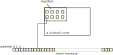
\includegraphics[width=\textwidth]{out/pdf/svg/cpu.pdf}
  \end{center}
\end{frame}

  %%%%%%%%%%%%%%%%%%%%%%%%%%%%%%%%%% 
\begin{frame}
  \frametitle{Memory}
  \begin{itemize}
  \item where majority of data your program processes are stored
  \item memory is essentially a large flat array indexed by
    integers, often called \ao{\it addresses}
  \item an address is just an integer
  \end{itemize}
    \begin{center}
    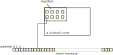
\includegraphics[width=0.8\textwidth]{out/pdf/svg/cpu.pdf}
  \end{center}
\end{frame}


  %%%%%%%%%%%%%%%%%%%%%%%%%%%%%%%%%% 
\begin{frame}[fragile]
  \frametitle{What a CPU (core) does}
  \begin{itemize}
  \item a special register, called \ao{\it program counter} or \ao{\it instruction pointer} specifies
    the address to fetch the next instruction at
  \item a CPU core is essentially a machine that does the following
    \begin{lstlisting}
repeat:
  inst = memory[@{\it program counter}@]
  execute inst
\end{lstlisting}
  \item an instrcution 
    \begin{itemize}
    \item performs some computation of values on a few registers or a memory location, and 
    \item changes the program counter (typically to the next instruction on memory)
    \end{itemize}
  \end{itemize}

  \begin{center}
    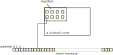
\includegraphics[width=0.45\textwidth]{out/pdf/svg/cpu.pdf}
  \end{center}
\end{frame}

  %%%%%%%%%%%%%%%%%%%%%%%%%%%%%%%%%% 
\begin{frame}[fragile]
  \frametitle{Exercise objectives}
  \begin{itemize}
  \item {\tt pl06\_how\_it\_gets\_compiled}
  \item learn how a \ao{compiler} does the job, 
  \item by inspecting assembly code generated from functions
    of the source language
  \end{itemize}
\end{frame}

%%%%%%%%%%%%%%%%%%%%%%%%%%%%%%%%%%
\section{A glance at x86 machine (assembly) code}
%%%%%%%%%%%%%%%%%%%%%%%%%%%%%%%%%% 

%%%%%%%%%%%%%%%%%%%%%%%%%%%%%%%%%% 
\begin{frame}[fragile]
  \frametitle{The first glance}
  \begin{columns}
    \begin{column}{0.6\textwidth}
  \begin{itemize}
  \item []
\begin{lstlisting}[escapechar=!,basicstyle=\tt\tiny]
    .file   "add123.go"
    .section    .go_export,"",@progbits

      ...

    .text
    .globl  go_0pl06.Add123
    .type   go_0pl06.Add123, @function
go_0pl06.Add123:
.LFB0:
    .cfi_startproc
    cmpq    %fs:112, %rsp
    jb      .L3
.L2:
    leaq    123(%rdi), %rax
    ret
.L3:
    movl    $0, %r10d
    movl    $0, %r11d
    call    __morestack
    ret
    jmp     .L2
    .cfi_endproc
.LFE0:
    .size   go_0pl06.Add123, .-go_0pl06.Add123
    .globl  go.pl06..types

      ...
\end{lstlisting}
\end{itemize}
\end{column}
\end{columns}
\begin{center}
looks scary?
\end{center}
\end{frame}

%%%%%%%%%%%%%%%%%%%%%%%%%%%%%%%%%% 
\begin{frame}[fragile]
  \frametitle{Unimportant lines}
  \begin{columns}
    \begin{column}{0.41\textwidth}
  \begin{itemize}
  \item []
\begin{lstlisting}[escapechar=!,basicstyle=\tt\tiny]
    !\hai{\tt .file   "add123.go"}!
    !\hai{\tt .section    .go\_export,"",@progbits}!

      ...

    !\hai{\tt .text}!
    !\hai{\tt .globl  go\_0pl06.Add123}!
    !\hai{\tt .type   go\_0pl06.Add123, @function}!
!\ao{\tt go\_0pl06.Add123:}!
!\ao{\tt .LFB0:}!
    !\hai{\tt .cfi\_startproc}!
    cmpq    %fs:112, %rsp
    jb      !\mura{.L3}!
!\ao{\tt .L2:}!
    leaq    123(%rdi), %rax
    ret
!\ao{\tt .L3:}!
    movl    $0, %r10d
    movl    $0, %r11d
    call    __morestack
    ret
    jmp     !\mura{.L2}!
    !\hai{\tt .cfi\_endproc}!
!\ao{\tt .LFE0:}!
    !\hai{\tt .size   go\_0pl06.Add123, ...}!
    !\hai{\tt .globl  go.pl06..types}!

      ...
\end{lstlisting}
\end{itemize}
\end{column}
    \begin{column}{0.59\textwidth}
      \begin{itemize}
      \item indented lines beginning with a dot
        (e.g., \hai{\tt .file, .section, .ascii, .text, .globl, } \ldots)
        are not instructions and \hai{\it largely not interesting or import}
      \item lines with a symbol followed by a colon
        (e.g., \ao{\tt .L2:, .LFE0:, go\_0pl06.Many\_\_args:,} \ldots)
        are \ao{\it labels} and used for the target of jump instructions
        or call instructions
      \end{itemize}
    \end{column}
  \end{columns}
\end{frame}


%%%%%%%%%%%%%%%%%%%%%%%%%%%%%%%%%% 
\begin{frame}[fragile]
  \frametitle{Where to look}
  \begin{columns}
    \begin{column}{0.41\textwidth}
  \begin{itemize}
  \item []
\begin{lstlisting}[escapechar=!,basicstyle=\tt\tiny]








!\ao{\tt go\_0pl06.Add123:}!
.LFB0:

    cmpq    %fs:112, %rsp
    jb      .L3
.L2:
    leaq    123(%rdi), %rax
    ret
.L3:
    movl    $0, %r10d
    movl    $0, %r11d
    call    __morestack
    ret
    jmp     .L2

.LFE0:



      ...
\end{lstlisting}
\end{itemize}
\end{column}
    \begin{column}{0.59\textwidth}
      \begin{itemize}
      \item focus on lines having \ao{\it instructins}
      \item instructions for a function start with a label
        \ao{\it similar to} the function name, but it may not be exactly the same (name mangling)
      \end{itemize}
    \end{column}
  \end{columns}
\end{frame}

%%%%%%%%%%%%%%%%%%%%%%%%%%%%%%%%%% 
\begin{frame}
  \frametitle{Registers}
\begin{itemize}
\item general-purpose 64 bit integer registers:
  \ao{\tt r\{a,b,c,d\}x}, \ao{\tt rdi}, \ao{\tt rsi}, \ao{\tt r[8-15]},
  \ao{\tt rbp}
\item general-purpose floating point number registers:
  \ao{\tt xmm[0-15]}
\item stack pointer register: \ao{\tt rsp}
\item a compare flag register: \ao{\tt eflags}, not directly used by instructions
  \begin{itemize}
  \item implicitly set by compare instructions
  \item implicitly used by conditional jump instructions
  \end{itemize}
\item an instruction pointer register: \ao{\tt rip},
  not directly used by instructions
  \begin{itemize}
  \item set by every instruction
  \end{itemize}
\item \url{https://wiki.cdot.senecapolytechnic.ca/wiki/X86_64_Register_and_Instruction_Quick_Start}
\end{itemize}
\end{frame}

%%%%%%%%%%%%%%%%%%%%%%%%%%%%%%%%%% 
\begin{frame}
  \frametitle{Frequently used instructions}
learn details and other instructions from the exercise    
\begin{itemize}
\item \ao{\tt addq} ($+$), \ao{\tt leaq} ($+$), \ao{\tt subq} ($-$), \ao{\tt imulq} ($\times$), \ao{\tt idivq} ($/$)
\item \ao{\tt movq} : move values between registers or between register and memory (load/store)
\item \ao{\tt cmpq} : compare two values and set the result into
  the \ao{\tt eflags} register
\item \ao{\tt jl} ($<$), \ao{\tt jle} ($\leq$), \ao{\tt jg} ($>$),
  \ao{\tt jge} ($\geq$), \ao{\tt je} ($=$), \ao{\tt jne} ($\neq$) :
  jump if a condition (indicated by \ao{\tt eflags}) is met
\item \ao{\tt call}, \ao{\tt ret} : call or return from a function
\end{itemize}
\end{frame}

%%%%%%%%%%%%%%%%%%%%%%%%%%%%%%%%%% 
\begin{frame}[fragile]
  \frametitle{How to read instructions and operands (of GNU assembler)}
  \begin{itemize}
  \item e.g., {\tt addq} instructios takes two operands
\begin{lstlisting}
addq @{\it x}@,@{\it y}@
\end{lstlisting}
and its effect is 
\begin{lstlisting}
@{\it y}@ += @{\it x}@
\end{lstlisting}
\item many two operand instructions behave similarly
\begin{lstlisting}
@\ao{\it op}@q @{\it x}@,@{\it y}@ @$\equiv$@ @{\it y}@ = @{\it y} \ao{\it op} {\it x}@
\end{lstlisting}
\item especially confusing is \ao{\tt subq}
\begin{lstlisting}
subq @{\it x}@,@{\it y}@ @$\equiv$@ @{\it y}@ = @{\it y}@ - @{\it x}@
\end{lstlisting}
\end{itemize}
\end{frame}

%%%%%%%%%%%%%%%%%%%%%%%%%%%%%%%%%% 
\begin{frame}
  \frametitle{Syntax of operands}
  \begin{itemize}
  \item \ao{{\tt \$}$n$} : immediate value of $n$
  \item \ao{{\tt \%}$R$} : register named $R$
  \item \ao{\tt (...)} : address operand (details in the next slide)
  \end{itemize}
  where
  \begin{itemize}
  \item $n$ : a constant ({\tt 4, 8,} etc.)
  \item $R$ : regiser name ({\tt rax, rbx, rdi,} etc.)
  \end{itemize}
  ex.
  \begin{itemize}
  \item \ao{\tt addq \$1,\%rax} : add 1 to {\tt \%rax} register
  \item \ao{\tt subq \$1,\%rax} : subtract 1 from {\tt \%rax} register
  \end{itemize}
\end{frame}

%%%%%%%%%%%%%%%%%%%%%%%%%%%%%%%%%% 
\begin{frame}
  \frametitle{Address operands}
  \begin{itemize}
  \item an address operand {\tt (...)} specifies an address,
    and can be
    \begin{itemize}
    \item \ao{\tt(\%$R$)} : $R$
    \item \ao{$n${\tt (\%$R$)}} : $R + n$
    \item \ao{$n${\tt (\%$R$,$s$,$R'$)}} : $R + s R' + n$
    \end{itemize}
  \item where
    \begin{itemize}
    \item $n, s$ : integer constants
    \item $R, R'$ : register names
    \end{itemize}
  \item ex.
    \begin{itemize}
    \item \ao{\tt mulq (\%rdi),\%rax} : reads address specified by {\tt \%rdi} and multiply {\tt \%rax} by it
    \item \ao{\tt movq \%rax,8(\%rdi)} : writes the value of {\tt \%rax} to the address specified by {\tt \%rdi+8}
    \item \ao{\tt leaq 16(\%rdi,8,\%rsi),\%rax} : {\tt \%rax = \%rdi + 8 * \%rsi + 16};
      this instruction looks like reading/writing memory, but
      it is actually just a peculiar arithmetic
      (common in address calculation but also used for integer addition)
    \end{itemize}
  \end{itemize}
\end{frame}

%%%%%%%%%%%%%%%%%%%%%%%%%%%%%%%%%% 
\begin{frame}[fragile]
  \frametitle{Julia assembly syntax}
  \begin{itemize}
  \item \aka{\it syntax and operand order actually differ between assemblers}
  \item they are of course identical in the binary level
  \item in particular, output from Julia ({\tt code\_native}) is different
    \begin{itemize}
    \item {\it destination-first syntax}
      \[ {\tt addq}\; x,y \quad \equiv \quad x\; \verb!+=!\; y \]

    \item address operands are more intuitive. ex.
    \end{itemize}
    {\small
      \begin{tabular}{|l|l|}\hline
        GNU                       & Julia \\\hline
        {\tt mulq (\%rdi),\%rax}  & {\tt mulq \%rax,[\%rdi]} \\
        {\tt movq \%rax,8(\%rdi)}  & {\tt movq [\%rdi+8],\%rax}      \\
        {\tt leaq 16(\%rdi,8,\%rsi),\%rax} & {\tt leaq \%rax,[\%rdi+8*\%rsi+16]}      \\\hline
      \end{tabular}}
  \end{itemize}
\end{frame}

%%%%%%%%%%%%%%%%%%%%%%%%%%%%%%%%%% 
\begin{frame}[fragile]
  \frametitle{Things to learn in the exercise}
  \begin{enumerate}
  \item {\bf calling convention or ABI :}
    function's incoming parameters and the return value
    are put in places (typically registers)
    predetermined by convention
    
  \item {\bf data representation :}
    once you know where incoming parameters and return values are,
    understand how data (integers, floating point numbers, structs,
    pointers to something, arrays, etc.) are represented, 
    by compiling simple functions that work on them. e.g.,
\begin{lstlisting}
f(a, i) = a[i]
\end{lstlisting}

\item {\bf control flow :}
  how various control flows (conditionals and loops) are implemented
  
\item {\bf function calls :}
  how function calls are implemented
\end{enumerate}
\end{frame}

\end{document}

%%%%%%%%%%%%%%%%%%%%%%%%%%%%%%%%%% 
\begin{frame}
  \frametitle{A method to learn assembly}
  \begin{itemize}
  \item you don't have to remember details
  \item ask details to the compiler
    \begin{itemize}
    \item {\tt gcc -S} generates assembly code
    \end{itemize}
  \end{itemize}
\end{frame}

%%%%%%%%%%%%%%%%%%%%%%%%%%%%%%%%%% 
\begin{frame}
  \frametitle{Major gaps you have to fill}
  \begin{itemize}
  \item a register $\approx$ a variable, but
    \begin{itemize}
    \item you have only a fixed number of them,
      so majority of values have to be stored in memory
    \item function parameters and return values are on
      predetermined registers ({\it calling convention}
      or {\it Application Binary Interface})
    \end{itemize}
  \item an instruction can perform only a single operation, so
    nested expressions (e.g., {\tt a * x + b * y + c * z}) must be
    broken down into a series of instructions
  \item there are no structured control flows (for, while, if, etc.);
    everything must be done by (conditional) jump instructions
    ($\approx$ ``goto'' statement)
  \end{itemize}
\end{frame}

  %%%%%%%%%%%%%%%%%%%%%%%%%%%%%%%%%% 
\ifja
\begin{frame}[fragile]
  \frametitle{コード生成 --- 人間コンパイラ内観}
  \begin{itemize}
  \item 例: 以下(ちなみに$\sqrt{c}$を求めるニュートン法)をどう機械語にするか
\begin{lstlisting}
double sq(double c, long n) {
  double x = c;
  for (long i = 0; i < n; i++) {
    x = x / 2 + c / (x + x);
  }
  return x;
}
\end{lstlisting}
\end{itemize}
\end{frame}
\fi

\ifen
\begin{frame}[fragile]
  \frametitle{Code generation by hand --- introspecting ``human compiler''}
  \begin{itemize}
  \item ex: how to convert the following (which finds $\sqrt{c}$ by the Newton method)
    into machine language 
\begin{lstlisting}
double sq(double c, long n) {
  double x = c;
  for (long i = 0; i < n; i++) {
    x = x / 2 + c / (x + x);
  }
  return x;
}
\end{lstlisting}
\end{itemize}
\end{frame}
\fi

%%%%%%%%%%%%%%%%%%%%%%%%%%%%%%%%%% 
\ifja
\begin{frame}[fragile]
  \frametitle{ステップ 1 --- 制御構造を goto だけに}
  \begin{columns}
    \begin{column}{0.48\textwidth}
  \begin{itemize}
  \item []
\begin{lstlisting}
double sq(double c, long n) {
  double x = c;
  for (long i = 0; i < n; i++) {
    x = x / 2 + c / (x + x);
  }
  return x;
}
\end{lstlisting}
\end{itemize}
\end{column}
\begin{column}{0.02\textwidth}
$\quad \Rightarrow $
\end{column}
\begin{column}{0.48\textwidth}
  \begin{itemize}
  \item []
\begin{lstlisting}
double sq(double c, long n) {
  double x = c;
  long i = 0;
  if (i >= n) goto Lend;
Lstart:
  x = x / 2 + c / (2 * x);
  i++;
  if (i < n) goto Lstart;
Lend:
  return x;
}
\end{lstlisting}
\end{itemize}
    \end{column}
  \end{columns}
\end{frame}
\fi

\ifen
\begin{frame}[fragile]
  \frametitle{Step 1 --- make all controls ``goto''s}
  \begin{columns}
    \begin{column}{0.48\textwidth}
  \begin{itemize}
  \item []
\begin{lstlisting}
double sq(double c, long n) {
  double x = c;
  for (long i = 0; i < n; i++) {
    x = x / 2 + c / (x + x);
  }
  return x;
}
\end{lstlisting}
\end{itemize}
\end{column}
\begin{column}{0.02\textwidth}
$\quad \Rightarrow $
\end{column}
\begin{column}{0.48\textwidth}
  \begin{itemize}
  \item []
\begin{lstlisting}
double sq(double c, long n) {
  double x = c;
  long i = 0;
  if (i >= n) goto Lend;
Lstart:
  x = x / 2 + c / (2 * x);
  i++;
  if (i < n) goto Lstart;
Lend:
  return x;
}
\end{lstlisting}
\end{itemize}
    \end{column}
  \end{columns}
\end{frame}
\fi

%%%%%%%%%%%%%%%%%%%%%%%%%%%%%%%%%% 
\ifja
\begin{frame}[fragile]
  \frametitle{ステップ 2 --- 式を C $=$ A op B に}
  \begin{columns}
    \begin{column}{0.47\textwidth}
  \begin{itemize}
  \item []
\begin{lstlisting}
double sq(double c, long n) {
  double x = c;
  long i = 0;
  if (i >= n) goto Lend;
Lstart:
  x = x / 2 + c / (2 * x);
  i++;
  if (i < n) goto Lstart;
Lend:
  return x;
}
\end{lstlisting}
\end{itemize}
\end{column}
\begin{column}{0.02\textwidth}
$\quad \Rightarrow $
\end{column}
\begin{column}{0.47\textwidth}
  \begin{itemize}
  \item []
\begin{lstlisting}
double sq3(double c, long n) {
  double x = c;
  long i = 0;
  if (!(i < n)) goto Lend;
Lstart:
  double @\ao{\tt t0}@ = 2;
  double @\ao{\tt t1}@ = x / t0;
  double @\ao{\tt t2}@ = t0 * x;
  double @\ao{\tt t3}@ = c / t2;
  x = t1 + t3;
  i = i + 1;
  if (i < n) goto Lstart;
 Lend:
  return x;
}
\end{lstlisting}
\end{itemize}
\end{column}
\end{columns}
\end{frame}
\fi

\ifen
\begin{frame}[fragile]
  \frametitle{Step 2 --- flatten all nested expressions to ``C $=$ A op B''}
  \begin{columns}
    \begin{column}{0.47\textwidth}
  \begin{itemize}
  \item []
\begin{lstlisting}
double sq(double c, long n) {
  double x = c;
  long i = 0;
  if (i >= n) goto Lend;
Lstart:
  x = x / 2 + c / (2 * x);
  i++;
  if (i < n) goto Lstart;
Lend:
  return x;
}
\end{lstlisting}
\end{itemize}
\end{column}
\begin{column}{0.02\textwidth}
$\quad \Rightarrow $
\end{column}
\begin{column}{0.47\textwidth}
  \begin{itemize}
  \item []
\begin{lstlisting}
double sq3(double c, long n) {
  double x = c;
  long i = 0;
  if (!(i < n)) goto Lend;
Lstart:
  double @\ao{\tt t0}@ = 2;
  double @\ao{\tt t1}@ = x / t0;
  double @\ao{\tt t2}@ = t0 * x;
  double @\ao{\tt t3}@ = c / t2;
  x = t1 + t3;
  i = i + 1;
  if (i < n) goto Lstart;
 Lend:
  return x;
}
\end{lstlisting}
\end{itemize}
\end{column}
\end{columns}
\end{frame}
\fi

%%%%%%%%%%%%%%%%%%%%%%%%%%%%%%%%%% 
\ifja
\begin{frame}[fragile]
  \frametitle{ステップ3 --- 変数に機械語レベルでの変数(レジスタまたはメモリ)を割り当て}
  \begin{itemize}
  \item 注: 浮動小数点数の定数は命令中には書けない
    / cannot embed floating point constants in instructions
\begin{lstlisting}
/* c : @\ao{\tt xmm0}@, n : @\ao{\tt rdi}@ */      
double sq3(double c, long n) {
  double x = c;       /* x : @\ao{\tt xmm1}@ */
  long i = 0;         /* i : @\ao{\tt rsi}@ */
  if (!(i < n)) goto Lend;
 Lstart:
  double t0 = 2;      /* t0 : @\ao{\tt xmm2}@ */
  double t1 = x / t0; /* t1 : @\ao{\tt xmm3}@ */
  double t2 = t0 * x; /* t2 : @\ao{\tt xmm4}@ */
  double t3 = c / t2; /* t3 : @\ao{\tt xmm5}@ */
  x = t1 + t3;
  i = i + 1;
  if (i < n) goto Lstart;
 Lend:
  return x;
}
\end{lstlisting}
\end{itemize}
\end{frame}
\fi

\ifen
\begin{frame}[fragile]
  \frametitle{Step 3 ---assign ``machine variables'' (registers or memory) to variables}
  \begin{itemize}
  \item note: cannot write floating point constants in instructions
\begin{lstlisting}
/* c : @\ao{\tt xmm0}@, n : @\ao{\tt rdi}@ */      
double sq3(double c, long n) {
  double x = c;       /* x : @\ao{\tt xmm1}@ */
  long i = 0;         /* i : @\ao{\tt rsi}@ */
  if (!(i < n)) goto Lend;
 Lstart:
  double t0 = 2;      /* t0 : @\ao{\tt xmm2}@ */
  double t1 = x / t0; /* t1 : @\ao{\tt xmm3}@ */
  double t2 = t0 * x; /* t2 : @\ao{\tt xmm4}@ */
  double t3 = c / t2; /* t3 : @\ao{\tt xmm5}@ */
  x = t1 + t3;
  i = i + 1;
  if (i < n) goto Lstart;
 Lend:
  return x;
}
\end{lstlisting}
\end{itemize}
\end{frame}
\fi

%%%%%%%%%%%%%%%%%%%%%%%%%%%%%%%%%% 
\ifja
\begin{frame}[fragile]
  \frametitle{ステップ4 --- 命令に変換}
  \begin{columns}
  \begin{column}{0.5\textwidth}
  \begin{itemize}
  \item []
\begin{lstlisting}
/* c : @\ao{\tt xmm0}@, n : @\ao{\tt rdi}@ */      
double sq3(double c, long n) {
 # double x = c;       /*x:xmm1*/
 movasd %xmm0,%xmm1
 # long i = 0;         /*i:rsi*/
 movq $0,%rsi
.Lstart:
 # if (!(i < n)) goto Lend;
 cmpq %rdi,%rsi  # n - i
 jle .Lend
 # double t0 = 2;      /*t0:xmm2*/
 movasd .L2(%rip),%xmm2
 # double t1 = x / t0; /*t1:xmm3*/
 movasd %xmm1,%xmm3
 divq %xmm2,%xmm3
 # double t2 = t0 * x; /*t2:xmm4*/
 movasd %xmm0,%xmm4
 mulsd xmm2,%xmm4
\end{lstlisting}%$
\end{itemize}
\end{column}

\begin{column}{0.48\textwidth}
\begin{itemize}
\item []
\begin{lstlisting}
 # double t3 = c/t2; /*t3:xmm5*/
 movasd %xmm0,%xmm5
 divsd %xmm4,%xmm5
 # x = t1 + t3;
 movasd %xmm3,%xmm1
 addsd %xmm5,%xmm1
 # i = i + 1;
 addq $1,%rsi
 # if (i < n) goto Lstart;
 cmpq %rdi,%rsi  # n - i
 jl .Lstart
.Lend:
 # return x;
 movq %xmm1,%xmm0
 ret
}
\end{lstlisting}%$
  \end{itemize}
\end{column}
\end{columns}
\end{frame}
\fi

\ifen
\begin{frame}[fragile]
  \frametitle{Step 4 --- convert them to machine instructions}
  \begin{columns}
  \begin{column}{0.5\textwidth}
  \begin{itemize}
  \item []
\begin{lstlisting}
/* c : @\ao{\tt xmm0}@, n : @\ao{\tt rdi}@ */      
double sq3(double c, long n) {
 # double x = c;       /*x:xmm1*/
 movasd %xmm0,%xmm1
 # long i = 0;         /*i:rsi*/
 movq $0,%rsi
.Lstart:
 # if (!(i < n)) goto Lend;
 cmpq %rdi,%rsi  # n - i
 jle .Lend
 # double t0 = 2;      /*t0:xmm2*/
 movasd .L2(%rip),%xmm2
 # double t1 = x / t0; /*t1:xmm3*/
 movasd %xmm1,%xmm3
 divq %xmm2,%xmm3
 # double t2 = t0 * x; /*t2:xmm4*/
 movasd %xmm0,%xmm4
 mulsd xmm2,%xmm4
\end{lstlisting}%$
\end{itemize}
\end{column}

\begin{column}{0.48\textwidth}
\begin{itemize}
\item []
\begin{lstlisting}
 # double t3 = c/t2; /*t3:xmm5*/
 movasd %xmm0,%xmm5
 divsd %xmm4,%xmm5
 # x = t1 + t3;
 movasd %xmm3,%xmm1
 addsd %xmm5,%xmm1
 # i = i + 1;
 addq $1,%rsi
 # if (i < n) goto Lstart;
 cmpq %rdi,%rsi  # n - i
 jl .Lstart
.Lend:
 # return x;
 movq %xmm1,%xmm0
 ret
}
\end{lstlisting}%$
  \end{itemize}
\end{column}
\end{columns}
\end{frame}
\fi

%%%%%%%%%%%%%%%%%%%%%%%%%%%%%%%%%% 
\ifja
\section{より一般の場合}
\fi
\ifen
\section{More general cases}
\fi
%%%%%%%%%%%%%%%%%%%%%%%%%%%%%%%%%% 
\ifja
\begin{frame}[fragile]
  \frametitle{コード生成 --- 一般的には難しいところ}
  \begin{itemize}
  \item 気軽に各途中結果にレジスタを割り当てたが \ldots
\begin{lstlisting}
  double x = c;       /* x : @\ao{\tt xmm1}@ */
Lstart:
  if (!(i < n)) goto Lend;
  double t0 = 2;      /* t0 : @\ao{\tt xmm2}@ */
  double t1 = x / t0; /* t1 : @\ao{\tt xmm3}@ */
  double t2 = t0 * x; /* t2 : @\ao{\tt xmm4}@ */
  double t3 = c / t2; /* t3 : @\ao{\tt xmm5}@ */
\end{lstlisting}
\item レジスタは足りなくなるかも知れない
\item 多くのレジスタは関数呼び出しをまたがると破壊される
\item オペランドレジスタが限定されている命令もある
  (e.g., 整数割り算の被除数は \%rax, \%rdx
  $\equiv$ \%rax, \%rdxは割り算をまたがると破壊される)
\item $\rightarrow$ 一般にはメモリ(スタック領域)も使う必要がある
  \end{itemize}
\end{frame}
\fi

\ifen
\begin{frame}[fragile]
  \frametitle{Things are more complex in general \ldots}
  \begin{itemize}
  \item we've liberally assign registers to intermediate results,
    but \ldots
\begin{lstlisting}
  double x = c;       /* x : @\ao{\tt xmm1}@ */
  Lstart:
  if (!(i < n)) goto Lend;
  double t0 = 2;      /* t0 : @\ao{\tt xmm2}@ */
  double t1 = x / t0; /* t1 : @\ao{\tt xmm3}@ */
  double t2 = t0 * x; /* t2 : @\ao{\tt xmm4}@ */
  double t3 = c / t2; /* t3 : @\ao{\tt xmm5}@ */
\end{lstlisting}
\item \mura{registers are finite (may run out)}
\item some registers are \mura{destroyed (i.e., values on them are lost) across a function call}
\item some instructions demand operands to be on \mura{specific registers}
  (e.g., dividend of integer division must be on {\tt rax} and {\tt rdx}
  $\equiv$ {\tt rax} and {\tt rdx} are destroyed across an integer division)
\item $\rightarrow$ you must use memory (``stack'' region) as well
  \end{itemize}
\end{frame}
\fi

%%%%%%%%%%%%%%%%%%%%%%%%%%%%%%%%%% 
\ifja
\begin{frame}
  \frametitle{最も単純だが一般的な(コンパイラによる)コード生成の作戦}
  \begin{itemize}
  \item 途中結果は一般にはメモリ(スタック領域)も使う必要がある
    $\Rightarrow$ 「常に」スタック領域を使うのが単純
  \end{itemize}
  \begin{center}
    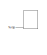
\includegraphics[width=0.5\textwidth]{out/pdf/lsvg/stack_1.pdf}
  \end{center}
\end{frame}
\fi

\ifen
\begin{frame}
  \frametitle{A simplest general strategy for code generation by a compiler}
  \begin{itemize}
  \item in general, memory (stack) must be used to hold intermediate results
    $\Rightarrow$ simply, \ao{{\it ``always''} use stack}
  \item a register is used only ``temporarily''
    (to read an operand from memory, which is immediately used by an instruction)
  \end{itemize}

  \begin{center}
    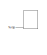
\includegraphics[width=0.5\textwidth]{out/pdf/lsvg/stack_1.pdf}
  \end{center}
\end{frame}
\fi

%%%%%%%%%%%%%%%%%%%%%%%%%%%%%%%%%% 
\ifja
\begin{frame}
  \frametitle{レジスタ使用慣例 (ABI)}
  \begin{itemize}
  \item 整数/ポインタの第1-6引数: rdi, rsi, rdx, rcx, r8, r9
  \item 浮動小数点数の引数は, xmm0, xmm1, \ldots 
  \item 整数/ポインタの返り値 : {\tt rax}
  \item rsp : 関数先頭でスタックの端を指し, そこには戻り番地が格納されている
  \item callee-save レジスタ: rbx, rbp, r12, r13, r14, r15
    (関数呼び出しをまたがって保存 $\rightarrow$
    呼び出された関数がそれらを使う場合は保存してから使う)
  \item その他のレジスタは caller-save
    (関数呼び出しをまたがったら壊れると仮定してコードを生成)
  \item 
    \url{https://wiki.cdot.senecacollege.ca/wiki/X86_64_Register_and_Instruction_Quick_Start}
    ``general-purpose registers'' を参照
  \end{itemize}
\end{frame}
\fi

\ifen
\begin{frame}
  \frametitle{Register usage conventions (ABI)}
  \begin{itemize}
  \item the first six integer/pointers arguments : \ao{\tt rdi, rsi, rdx, rcx, r8, r9}
  \item floating point number arguments : \ao{\tt xmm0, xmm1, \ldots}
  \item an integer/pointer return value : \ao{\tt rax}
  \item {\tt rsp} : points the end of the stack upon function entry, which holds the return address
  \item callee-save registers: \ao{\tt rbx, rbp, r12, r13, r14, r15}
    (preserved across function calls $\rightarrow$
    a function must save them before using (setting a value to) them)
  \item other registers are caller-save
    (a function must assume they are destroyed across function calls)
  \item see ``general-purpose'' registers in
    \url{https://wiki.cdot.senecacollege.ca/wiki/X86_64_Register_and_Instruction_Quick_Start}
  \end{itemize}
\end{frame}
\fi

%%%%%%%%%%%%%%%%%%%%%%%%%%%%%%%%%% 
\ifja
\begin{frame}
  \frametitle{関数呼び出し時の動き}
  \begin{itemize}
  \item {\tt long f() \{ ... g(1,2,3,4,5,6,7,8); ... \}}
  \item
    \only<1>{f実行中}%
    \only<2>{{\tt call g}実行直前 {\scriptsize rdi=1, rsi=2, rdx=3, rcx=4, r8=5, r9=6}}% 
    \only<3>{{\tt call g}実行直後({\tt g}開始)}%
    \only<4>{{\tt g}が使うcallee-saveレジスタ保存}
    \only<5>{{\tt g}実行中}
  \item []
\begin{center}
  \only<1>{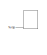
\includegraphics[height=0.8\textheight]{out/pdf/lsvg/stack_1.pdf}}%
  \only<2>{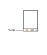
\includegraphics[height=0.8\textheight]{out/pdf/lsvg/stack_2.pdf}}%
  \only<3>{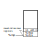
\includegraphics[height=0.8\textheight]{out/pdf/lsvg/stack_3.pdf}}%
  \only<4>{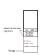
\includegraphics[height=0.8\textheight]{out/pdf/lsvg/stack_4.pdf}}%
  \only<5>{\includegraphics[height=0.8\textheight]{out/pdf/lsvg/stack_5.pdf}}
\end{center}
\end{itemize}
\end{frame}
\fi

\ifen
\begin{frame}
  \frametitle{What happens upon function calls}
  \begin{itemize}
  \item {\tt long f() \{ ... g(1,2,3,4,5,6,7,8); ... \}}
  \item
    \only<1>{during {\tt f}}%
    \only<2>{right before ``{\tt call g}'' {\tt {\scriptsize rdi=1, rsi=2, rdx=3, rcx=4, r8=5, r9=6}}}% 
    \only<3>{right after ``{\tt call g}'' (when {\tt g} started)}%
    \only<4>{save callee-save registers {\tt g} uses}
    \only<5>{during {\tt g}}
  \item []
\begin{center}
  \only<1>{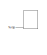
\includegraphics[height=0.8\textheight]{out/pdf/lsvg/stack_1.pdf}}%
  \only<2>{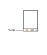
\includegraphics[height=0.8\textheight]{out/pdf/lsvg/stack_2.pdf}}%
  \only<3>{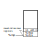
\includegraphics[height=0.8\textheight]{out/pdf/lsvg/stack_3.pdf}}%
  \only<4>{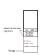
\includegraphics[height=0.8\textheight]{out/pdf/lsvg/stack_4.pdf}}%
  \only<5>{\includegraphics[height=0.8\textheight]{out/pdf/lsvg/stack_5.pdf}}
\end{center}
\end{itemize}
\end{frame}
\fi

%%%%%%%%%%%%%%%%%%%%%%%%%%%%%%%%%% 
\ifja
\begin{frame}[fragile]
  \frametitle{関数呼び出しを含むコード生成例}

  \begin{itemize}
  \item []
\begin{lstlisting}
double integ(long n) {
  double x = 0;
  double dx = 1 / (double)n;
  double s = 0;
  for (long i = 0; i < n; i++) {
    s += f(x);
    x += dx;
  }
  return s * dx;
}
\end{lstlisting}
\end{itemize}

\end{frame}
\fi

\ifen
\begin{frame}[fragile]
  \frametitle{Code generation including function calls}
  \begin{itemize}
  \item []
\begin{lstlisting}
double integ(long n) {
  double x = 0;
  double dx = 1 / (double)n;
  double s = 0;
  for (long i = 0; i < n; i++) {
    s += f(x);
    x += dx;
  }
  return s * dx;
}
\end{lstlisting}
  \end{itemize}
\end{frame}
\fi

%%%%%%%%%%%%%%%%%%%%%%%%%%%%%%%%%% 
\ifja
\begin{frame}[fragile]
  \frametitle{``goto''化と``C = A op B''化}
  \begin{itemize}
  \item []
\begin{lstlisting}
double integ3(long n) {    /*  n :  @\ao{\tt 0(\%rsp)}@ */
  double x = 0;            /*  x :  @\ao{\tt 8(\%rsp)}@ */
  double t0 = 1;           /* t0 : @\ao{\tt 16(\%rsp)}@ */
  double t1 = (double)n;   /* t1 : @\ao{\tt 24(\%rsp)}@ */
  double dx = t0 / t1;     /* dx : @\ao{\tt 32(\%rsp)}@ */
  double s = 0;            /*  s : @\ao{\tt 40(\%rsp)}@ */
  long i = 0;              /*  i : @\ao{\tt 48(\%rsp)}@ */
  if (!(i < n)) goto Lend;
 Lstart:
  double t2 = f(x);        /* t2 : @\ao{\tt 56(\%rsp)}@ */
  s += t2;
  x += dx;
  i += 1;
  if (i < n) goto Lstart;
  Lend:
  double t3 = s * dx;      /* t3 : @\ao{\tt 64(\%rsp)}@ */
  return t3;
}
\end{lstlisting}
  \end{itemize}
\end{frame}
\fi

\ifen
\begin{frame}[fragile]
  \frametitle{converting to ``goto''s and ``C = A op B''s}
  \begin{itemize}
  \item []
\begin{lstlisting}
double integ3(long n) {    /*  n :  @\ao{\tt 0(\%rsp)}@ */
  double x = 0;            /*  x :  @\ao{\tt 8(\%rsp)}@ */
  double t0 = 1;           /* t0 : @\ao{\tt 16(\%rsp)}@ */
  double t1 = (double)n;   /* t1 : @\ao{\tt 24(\%rsp)}@ */
  double dx = t0 / t1;     /* dx : @\ao{\tt 32(\%rsp)}@ */
  double s = 0;            /*  s : @\ao{\tt 40(\%rsp)}@ */
  long i = 0;              /*  i : @\ao{\tt 48(\%rsp)}@ */
  if (!(i < n)) goto Lend;
 Lstart:
  double t2 = f(x);        /* t2 : @\ao{\tt 56(\%rsp)}@ */
  s += t2;
  x += dx;
  i += 1;
  if (i < n) goto Lstart;
  Lend:
  double t3 = s * dx;      /* t3 : @\ao{\tt 64(\%rsp)}@ */
  return t3;
}
\end{lstlisting}
  \end{itemize}
\end{frame}
\fi

%%%%%%%%%%%%%%%%%%%%%%%%%%%%%%%%%% 
\begin{frame}[fragile]
  \frametitle{機械語 / Machine code}
  \begin{columns}
    \begin{column}{0.49\textwidth}
  \begin{itemize}
  \item []
\begin{lstlisting}
double integ3(long n) {
  /* n : 0(%rsp) */
  movq %rdi,0(%rsp)  
  # double x = 0;
  /* x : 8(%rsp)*/
  movsd .L0(%rip),%xmm0
  movsd %xmm0,8(%rsp)
  # double t0 = 1;
  /* t0 : 16(%rsp)*/
  movq $1,16(%rsp)
  # double t1 = (double)n;
  /* t1 : 24(%rsp)*/
  cvtsi2sdq 0(%rsp),%xmm0
  movsd %xmm0,24(%rsp)
  # double dx = t0 / t1;
  /* dx : 32(%rsp) */
  movsd 16(%rsp),%xmm0
  divsd 24(%rsp),%xmm0
  movsd %xmm0,32(%rsp)
  # double s = 0;
  /* s : 40(%rsp) */
  movsd .L0(%rip),%xmm0
  movsd %xmm0,40(%rsp)
\end{lstlisting}%$
  \end{itemize}
    \end{column}
    \begin{column}{0.49\textwidth}
  \begin{itemize}
  \item []
\begin{lstlisting}
  # long i = 0;
  /* i : 48(%rsp) */
  movq $0,48(%rsp)
  # if (!(i < n)) goto Lend;
  movq 0(%rsp),%rdi
  cmpq 48(%rsp),%rdi # n - i
  jle .Lend
.Lstart:
  # double t2 = f(x);
  /* t2 : 56(%rsp) */
  movq 8(%rsp),%rdi
  call f
  movq %rax,56(%rsp)
  # s += t2;
  movq 40(%rsp),%xmm0
  addsd 56(%rsp),%xmm0
  movq %xmm0,40(%rsp)
  # x += dx;
  movsd 8(%rsp),%xmm0
  addsd 32(%rsp),%xmm0
  movsd %xmm0,8(%rsp)
\end{lstlisting}%$
\end{itemize}
\end{column}
\end{columns}
  
\end{frame}


%%%%%%%%%%%%%%%%%%%%%%%%%%%%%%%%%% 
\begin{frame}[fragile]
  \frametitle{機械語 / Machine code}
  \begin{columns}
    \begin{column}{0.49\textwidth}
  \begin{itemize}
  \item []
\begin{lstlisting}
  # i += 1;
  movq 48(%rsp),%rdi
  addq $1,%rdi
  movq %rdi,48(%rsp)
  # if (i < n) goto Lstart;
  movq 0(%rsp),%rdi
  cmpq 48(%rsp),%rdi # n - i
  jg .Lstart
.Lend:
  movsd 40(%rsp),%xmm0
  addsd 32(%rsp),%xmm0
  addsd %xmm0,64(%rsp)
  # return t3;
  addsd 64(%rsp),%xmm0
  ret
}
\end{lstlisting}%$
  \end{itemize}
    \begin{column}{0.49\textwidth}
\phantom{aaa}
\end{column}
    \end{column}
\end{columns}
\end{frame}

%%%%%%%%%%%%%%%%%%%%%%%%%%%%%%%%%% 
\ifja
\section{最小限のCからのコード先生器}
\fi
\ifen
\section{Implementing a minimum compiler for a C-like language}
\fi
%%%%%%%%%%%%%%%%%%%%%%%%%%%%%%%%%% 
\ifja
\begin{frame}
  \frametitle{コード生成器 --- 演習での前提}
  \begin{itemize}
  \item 型は \ao{long (8 バイト整数)のみ}
    \begin{itemize}
    \item したがって typedef なども無し
    \item int もなし, 浮動小数点数もポインタもなし
    \item 全部longだから静的な型検査もいらない
    \end{itemize}
  \item \ao{大域変数もなし} $\Rightarrow$
    \begin{itemize}
    \item \ao{プログラム $=$ 関数定義のリスト}
    \end{itemize}
  \item ややこしい文は if, while, 複合文 (\{ \ldots\ \}) のみ
  \item 変数宣言は複合文の先頭で, 初期化の式もなし
  \item 以上は字句の定義(cc\_lex.mll),
    文法の定義(cc\_parse.mly)に反映されている
  \end{itemize}
\end{frame}
\fi

\ifen
\begin{frame}
  \frametitle{Spec overview}
  \begin{itemize}
  \item this will be your final report if you choose option 0
  \item all expressions have type \ao{\tt long (8 byte integers)}
    \begin{itemize}
    \item no \mura{\tt typedef}s
    \item no \mura{{\tt int}s, floating point numbers, or pointers}
    \item everything is long, so \mura{type checks} are unnecessary
    \end{itemize}
  \item \ao{no global variables} $\Rightarrow$
    \begin{itemize}
    \item \ao{a program $=$ list of function definitions}
    \end{itemize}
  \item function calls with C conventions, so you can call or be called by C functions
    compiled by ordinary compilers (e.g., gcc)
  \item supported complex statements are \ao{\tt if, while} and \ao{compound statement ({\tt \{ \ldots\ \}})} only
  % \item all variable definitions must come at the beginning of a block and
  %   initializes ({\tt long} $x$ {\tt = } {\it expr}) are not supported
  % \item they are expressed in token definitions ({\tt cc\_lex.mll}),
  %   and grammar definitions ({\tt cc\_parse.mly})
  \end{itemize}
\end{frame}
\fi

\iffalse
\ifen
\begin{frame}
  \frametitle{Detailed spec will come soon}
  \begin{itemize}
  \item I will give you (a part of)
    \begin{itemize}
    \item definition of an abstract syntax tree (AST)
    \item the grammar and a parser (source program $\rightarrow$ AST)
    \end{itemize}
  \item so that you can mainly work on the code generator (AST $\rightarrow$ assembly)
  \item bonus points will be given to extensions and optimizations
    \begin{itemize}
    \item other data types (floating point numbers and arrays/pointers)
    \item advanced control flows
    \item better register usage
    \item etc.
    \end{itemize}
  \end{itemize}
\end{frame}
\fi
\fi

\ifen
\begin{frame}
  \frametitle{Structure of the program}
  \begin{itemize}
  \item {\tt parser/}
    \begin{itemize}
    \item {\tt minc\_grammar.y} --- grammar definition
    \item {\tt minc\_to\_xml.py} --- minC $\rightarrow$ XML converter
    \end{itemize}
  \item {\tt \{ml,jl,go,rs\}/minc/}
    \begin{itemize}
    \item {\tt minc\_ast.??} --- abstract syntax tree (AST) definition
    \item {\tt minc\_parse.??} --- grammar definition
    \item \ao{\tt minc\_cogen.??} --- code generation from AST
    \item {\tt main.??} or {\tt minc.??} --- main driver
    \end{itemize}
  \item the exact location depends on the language
  \item your work will be mostly done in \ao{\tt minc\_cogen.??}
  \end{itemize}
\end{frame}
\fi

\ifen
\begin{frame}[fragile]
  \frametitle{Abstract Syntax Tree (AST)}
  \begin{itemize}
  \item naturally represent a program
    \begin{itemize}
    \item the whole program
    \item function definition
    \item statement
    \item expression
    \item etc.
    \end{itemize}
  \item see {\tt minc\_ast.??}
  \end{itemize}
\end{frame}
\fi

\ifen
\begin{frame}
  \frametitle{Code generation ({\tt minc\_cogen}) --- basic structure}
  \begin{itemize}
  \item takes a parse tree (AST) and returns machine code
    (a list of instructions)
  \item generate machine code for an AST 
    $\approx$ generate machine code of its components and properly arrange them

  \item the program ({\tt program}) $\rightarrow$ function definition
    ({\tt definition})
    $\rightarrow$ statement ({\tt stmt}) $\rightarrow$ expression ({\tt expr})
    
  \item code generator has lots of
    \begin{itemize}
    \item case analysis based on the type of the tree; use
      \begin{itemize}
      \item pattern matching (OCaml match and Rust match) or
      \item polymorphism (OCaml objects, Julia function, Go interface, Rust trait)
      \end{itemize}
    \item recursive calls to child trees
    \end{itemize}
  \end{itemize}
\end{frame}
\fi

\ifen
\begin{frame}[fragile]
  \frametitle{Compiling an entire file}
  \begin{itemize}
  \item $\approx$ concatenate compilation of individual function definitions
  \end{itemize}
  \begin{columns}
    \begin{column}{0.45\textwidth}
      \includegraphics[width=0.9\textwidth]{out/pdf/lsvg/translate_1.pdf}
    \end{column}
    \begin{column}{0.55\textwidth}
In OCaml, it will look like \ldots
\begin{lstlisting}[escapechar=!]
let ast_to_insns_program defs ... =
  List.concat (List.map (fun def -> !\ao{\tt ast\_to\_insns\_def}! def ...) defs)
\end{lstlisting}
    \end{column}
  \end{columns}
\end{frame}
\fi

\ifen
\begin{frame}[fragile]
  \frametitle{Compiling a function definition}
  \begin{itemize}
  \item $\approx$ compile the body (statement); put
    prologue (grow the stack, etc.) and epilogue
    (shrink the stack, ret, etc.)
  \end{itemize}
  \begin{columns}
    \begin{column}{0.45\textwidth}
      \includegraphics[width=0.9\textwidth]{out/pdf/lsvg/translate_2.pdf}
    \end{column}
    \begin{column}{0.55\textwidth}
\begin{lstlisting}[escapechar=!]
let ast_to_insns_def def ... =
  match def with
    DefFun(f, params, ret_type, body) ->
      (gen_prologue def)
      @ (!\ao{\tt ast\_to\_insns\_stmt}! body ...)
      @ (gen_epilogue def)
\end{lstlisting}
    \end{column}
  \end{columns}
\end{frame}
\fi

\ifen
\begin{frame}[fragile]
  \frametitle{Compiling a statement (e.g., {\tt while} statement)}
  \begin{itemize}
  \item $\approx$ place compilation of the condition expression and the body
    as follows. add a conditional to determine if the loop continues
  \end{itemize}
  \begin{columns}
    \begin{column}{0.45\textwidth}
      \includegraphics[width=0.9\textwidth]{out/pdf/lsvg/translate_3.pdf}
    \end{column}
    \begin{column}{0.55\textwidth}
\begin{lstlisting}[escapechar=!]
let rec ast_to_insns_stmt stmt ...  =
  match stmt with
    ...
  | StmtWhile(cond, body) ->
    let cond_op,cond_insns = !\ao{\tt ast\_to\_insns\_expr}! cond ... in
    let body_insns = !\ao{\tt ast\_to\_insns\_stmt}! body ... in
    let ... in
    [ jmp Lc;
      Ls ]
    @ body_insns
    [ Lc ]
    @ cond_insns @
    [ cmpq $0,cond_op;
      jne Ls ]
\end{lstlisting} %$
    \end{column}
  \end{columns}
\end{frame}
\fi

\ifen
\begin{frame}[fragile]
  \frametitle{Compiling an expression (arithmetic)}
  \begin{itemize}
  \item $\approx$ compile the arguments; an arithmetic instruction
  \end{itemize}
  \begin{columns}
    \begin{column}{0.43\textwidth}
\includegraphics[width=0.9\textwidth]{out/pdf/lsvg/translate_4.pdf}
    \end{column}
    \begin{column}{0.57\textwidth}
\begin{lstlisting}[escapechar=!]
let rec ast_to_insns_expr expr ... =
  match expr with
    ...
  | ExprOp("+", [e0; e1]) ->
    let insns1,op1 = !\ao{\tt ast\_insns\_expr}! e1 ... in
    let insns0,op0 = !\ao{\tt ast\_insns\_expr}! e0 ... in
    let m = !{\it a slot on the stack}! in
    ((insns1
    @ [ movq op1,m ]
    @ insns0
    @ [ addq m,op0 ]), (* op0 = op0 + m *)
    op0)
  | ...
\end{lstlisting}
    \end{column}
  \end{columns}
  {\footnotesize
    \begin{itemize}
    \item Remark: {\tt movq XX(\%rsp),...} saves
      the first operand, ensuring
      it won't be destroyed during the evaluation of
      the second
    \item remember we are following the simplest strategy
      $=$ ``save all intermediate results on the stack''
    \end{itemize}
  }
\end{frame}
\fi

\ifen
\begin{frame}[fragile]
  \frametitle{Compiling an expression (comparison)}
  \begin{itemize}
  \item $A$ {\tt <} $B$ is an expression that evaluates to
    \begin{itemize}
    \item 1 if $A$ {\tt <} $B$
    \item 0 if $A$ {\tt >=} $B$
    \end{itemize}
  \item no single instruction exactly does this
  \item note that they can appear anywhere expression can
    \begin{itemize}
    \item {\tt z = x < y}, {\tt (x < y) + z}, and {\tt f(x < 1)} are allowed
      (they do not necessarily appear in condition expression of
      {\tt if} or {\tt while})
    \end{itemize}
  \item how to do it in assembly code?
    \begin{enumerate}
    \item conditional branch
    \item \ao{\it conditional set instruction}. e.g.,
\begin{lstlisting}
movq $0,%rax
cmpq %rdi,%rsi
setle %al  
\end{lstlisting}%$
will set
{\tt \%al} (the lowest 8 bits of {\tt \%rax}) to 1
when {\tt \%rsi - \%rdi} $\leq$ 0 (less-than-or-equal)
    \end{enumerate}
  \end{itemize}
\end{frame}
\fi

\ifen
\begin{frame}[fragile]
  \frametitle{Compiling an expression (comparison)}
  \begin{itemize}
  \item $\approx$ compile the arguments; compare; conditional set
  \end{itemize}
  
  \begin{columns}
    \begin{column}{0.43\textwidth}
\includegraphics[width=0.9\textwidth]{out/pdf/lsvg/translate_5.pdf}
    \end{column}
    \begin{column}{0.57\textwidth}
\begin{lstlisting}[escapechar=!]
let rec ast_to_insns_expr expr ... =
  match expr with
    ...
  | ExprOp("<", [e0; e1]) ->
    let insns1,op1 = !\ao{\tt ast\_to\_insns\_expr}! e1 ... in
    let insns0,op0 = !\ao{\tt ast\_to\_insns\_expr}! e0 ... in
    let m0 = !{\it a slot on the stack}! in
    let m1 = !{\it a slot on the stack}! in
      ...
    ((insns1
      @ [ movq op1,m1 ]
      @ insns0
      @ [ movq op0,m0;
          movq $0,%rax;
          movq m0,op0;
          cmpq m1,op0;
          setl rax ]
    op0)
  | ...
\end{lstlisting} %$
    \end{column}
  \end{columns}

\end{frame}
\fi

\ifen
\begin{frame}[fragile]
  \frametitle{Compiling an expression (function call)}
  \begin{itemize}
  \item $\approx$ compile all arguments; put them to positions specified by ABI; a {\tt call} instruction
  \end{itemize}
  \begin{columns}
\begin{column}{0.45\textwidth}
\includegraphics[width=0.9\textwidth]{out/pdf/lsvg/translate_6.pdf}
\end{column}
\begin{column}{0.5\textwidth}
\begin{lstlisting}[escapechar=!]
let rec ast_to_insns_expr expr ... =
  match expr with
    ...
  | ExprCall(f, args) ->
     let insns,arg_vars = !\ao{\tt ast\_to\_insns\_exprs}! args env var_idx in
     ((insns @ (make_call f arg_vars)), rax)
\end{lstlisting}
\end{column}
\end{columns}
\end{frame}
\fi

\ifen
\begin{frame}[fragile]
  \frametitle{Details we have been leaving out}
  \begin{itemize}
  \item how to determine locations
    to save values of \ao{\it subexpressions} and \mura{\it variables}
  \item that is, how to determine XX below
    \begin{center}
    \includegraphics[width=0.5\textwidth]{out/pdf/lsvg/translate_4.pdf}
  \end{center}
\end{itemize}
\end{frame}
\fi
\ifen
\begin{frame}[fragile]
  \frametitle{Determining where to save subexpressions}
  \begin{itemize}
\item {\tt ast\_to\_insns\_expr} receives a value ($v$)
  pointing to the lowest end of free space
\item []
  {\tt ast\_to\_insns\_expr} $E$ {\it v} \ldots 
  generates instructions that evaluate $E$ using
  (destroying) only addresses above $v${\tt (\%rsp)}
\item $\rightarrow$ when evaluating \aka{\fbox{$A$}} + \ao{\fbox{$B$}},
  save \ao{\fbox{$B$}} at $v${\tt (\%rsp)}
\item let \aka{\fbox{$A$}} use $v + 8$ and higher addresses
\end{itemize}

  \begin{columns}
    \begin{column}{0.34\textwidth}
      \includegraphics[width=0.9\textwidth]{out/pdf/lsvg/translate_4.pdf}
    \end{column}
    \begin{column}{0.66\textwidth}
\begin{lstlisting}[escapechar=!]
let rec ast_to_insns_expr expr !\ao{$v$}! =
 match expr with
  ...
 | ExprOp("+", e0, e1) ->
  let insns1,op1 = !\ao{\tt ast\_to\_insns\_expr}! e1 !\ao{$v$}! .. in
  let insns0,op0 = !\ao{\tt ast\_to\_insns\_expr}! e0 (!\underline{\tt \ao{$v$} + 8}!) .. in
  let m = !\ao{$v$}!(%rsp) in
  ((insns1
  @ [ movq op1,m ]
  @ insns0
  @ [ addq m,op0 ]), (* op0 = op0 + m *)
  op0)
 | ...
\end{lstlisting}
    \end{column}    
  \end{columns}

\end{frame}
\fi

\ifen
\begin{frame}[fragile]
  \frametitle{Locations to hold variables}
  \begin{itemize}
  \item ex:
\begin{lstlisting}
if (...) {
  long a, b, c;
  ...
}
\end{lstlisting}
\item we need to hold {\tt a, b, c} on the stack
\item the problem is almost identical to saving values of subexpressions
\item $\rightarrow$
  {\tt ast\_to\_insns\_stmt} also takes {\it v} pointing to the beginning of
  the free space
\item [] spec: {\tt ast\_to\_insns\_stmt} $S$ $v$ \ldots generates
  instructions to execute $S$; they use (destroy)
  only addresses above $v${\tt (\%rsp)}
\item $\rightarrow$ e.g., hold
  ${\tt a} \mapsto v${\tt (\%rsp)}, 
  ${\tt b} \mapsto v+8${\tt (\%rsp)}, 
  ${\tt c} \mapsto v+16${\tt (\%rsp)} 
\end{itemize}
\end{frame}
\fi

\ifen
\begin{frame}[fragile]
  \frametitle{Environment: records where variables are held}
  \begin{itemize}
  \item when a variable occurs in an expression,
    we need to get the location that holds the variable
    \begin{itemize}
    \item ex: to compile {\tt x + 1}, we need to know where {\tt x} is held
    \end{itemize}
  \item make a data structure that holds
    a mapping ``variable $\mapsto$ location'' \ao{\it (environment)}
    and pass it to {\tt ast\_to\_insns\_stmt} and {\tt ast\_to\_insns\_expr}
  \item when new variables are declared at the beginning of
    a compound statement (\{ \ldots \}), add new mappings to it
  \end{itemize}
\end{frame}
\fi

\ifen
\begin{frame}[fragile]
  \frametitle{{\tt ast\_to\_insns\_expr} receives an environment}
  \begin{itemize}
  \item []
\begin{lstlisting}[escapechar=!]
let rec ast_to_insns_expr expr !\ao{\it env}! !\ao{$v$}! =
  match expr with
    ...
  | ExprId(x) ->
     let loc = env_lookup x !\ao{\it env}! in
     ([ movq loc,... ], ...)
  | ...
\end{lstlisting}
\item {\tt env\_lookup} {\it x} {\it env} searches
  environment {\it env} for $x$ and returns its location
\end{itemize}
\end{frame}
\fi

\ifen
\begin{frame}[fragile]
  \frametitle{{\tt ast\_to\_insns\_stmt} receives an environment too}
  \begin{itemize}
  \item []
\begin{lstlisting}[escapechar=!]
let rec ast_to_insns_stmt expr !\ao{\it env}! !\ao{$v$}! =
  match expr with
    ...
  | StmtCompound(decls, stmts) ->
     let env',v' = env_extend decls !\ao{\it env}! !\ao{$v$}! in
     cogen_stmts stmts env' v' ...
  | ...
\end{lstlisting}
\item {\tt env\_extend} {\it decls} {\it env} $v$
  \begin{itemize}
  \item assign locations ($v$, $v+8$, $v+16$, \ldots)
    to variables declared in {\it decls}
  \item register them in {\it env}
  \item return the new environment {\it env'} and the new free space {\it v'}
  \end{itemize}
\end{itemize}
\end{frame}
\fi

\ifen
\begin{frame}[fragile]
  \frametitle{Implementing environment}
  \begin{itemize}
  \item an environment is a list of (variable name, location)'s
  \item {\it loc} {\tt = env\_lookup} $x$ {\it env}
    \begin{itemize}
    \item []
      returns the location paired with $x$ in environment {\it env}
    \end{itemize}
  \item {\it env'} {\tt = env\_add} $x$ {\it loc} {\it env}
    \begin{itemize}
    \item []
      returns a new environment {\it env'} which has a new
      mapping $x \mapsto$ {\it loc} in addition to {\it env}
      ({\tt ($x$, {\it loc})::{\it env}})
    \end{itemize}
  \item an environment can be easily implemented with a list of (variable name, location)'s
    and is left for your exercise
  \end{itemize}
\end{frame}
\fi

\end{document}
%%%%%%%%%%%%%%%%%%%%%%%%%%%%%%%%%% 
\ifja
\begin{frame}
  \frametitle{プログラムの構成}
  \begin{itemize}
  \item {\tt cc\_ast.ml} --- 構文木定義
  \item {\tt cc\_parse.mly} --- 文法定義
  \item {\tt cc\_lex.mll} --- 字句定義
  \item \ao{\tt cc\_cogen.ml} --- 構文木からコード生成
  \item {\tt cc.ml} --- メイン
  \end{itemize}

  演習のほとんどの部分は, \ao{\tt cc\_cogen.ml}で行われるだろう
\end{frame}
\fi

\ifen
\begin{frame}
  \frametitle{Structure of the program}
  \begin{itemize}
  \item {\tt cc\_ast.ml} --- abstract syntax tree (AST) definition
  \item {\tt cc\_parse.mly} --- grammar definition
  \item {\tt cc\_lex.mll} --- lexer definition
  \item \ao{\tt cc\_cogen.ml} --- code generation from AST
  \item {\tt cc.ml} --- main driver
  \end{itemize}

  your work in this exercise will be mostly done in \ao{\tt cc\_cogen.ml}
  
\end{frame}
\fi

%%%%%%%%%%%%%%%%%%%%%%%%%%%%%%%%%% 
\ifja
\begin{frame}[fragile]
  \frametitle{構文木定義 ({\tt cc\_ast.ml}) --- 関数定義}
  \begin{itemize}
  \item Cの関数定義の例
\begin{lstlisting}
@\ao{\tt long}@ @\mido{\tt f}@ (@\mura{\tt long x, long y}@) {
  return x + y;
}
\end{lstlisting}
\item $\Rightarrow$ 関数定義の構文木の定義
\begin{lstlisting}
type definition =
  FUN_DEF of (@\ao{\tt type\_expr}@ * @\mido{\tt string}@ * @\mura{\tt (type\_expr * string) list}@ * stmt) 
\end{lstlisting}
  \end{itemize}
\end{frame}
\fi

\ifen
\begin{frame}[fragile]
  \frametitle{AST ({\tt cc\_ast.ml}) --- function definition}
  \begin{itemize}
  \item an example C function definition
\begin{lstlisting}
@\ao{\tt long}@ @\mido{\tt f}@ (@\mura{\tt long x, long y}@) {
  return x + y;
}
\end{lstlisting}
\item $\Rightarrow$ AST definition for function definition
\begin{lstlisting}
type definition =
  FUN_DEF of (@\ao{\tt type\_expr}@ * @\mido{\tt string}@ * @\mura{\tt (type\_expr * string) list}@ * stmt) 
\end{lstlisting}
  \end{itemize}
\end{frame}
\fi
%%%%%%%%%%%%%%%%%%%%%%%%%%%%%%%%%% 
\ifja
\begin{frame}[fragile]
  \frametitle{構文木の定義 --- 文}
  \begin{itemize}
\item if文
\begin{lstlisting}
if (@\ao{\tt x < y}@) @\mido{\tt \{ x++; return x; \} }@ else @\mura{\tt return y;}@
\end{lstlisting}
$\Rightarrow$
\begin{lstlisting}
STMT_IF of (@\ao{\tt expr}@ * @\mido{\tt stmt}@ * @\mura{\tt stmt}@)
\end{lstlisting}

\item 複合文
\begin{lstlisting}
{ @\ao{\tt long r;}@ @\mido{\tt if (x < y) r = 10; else r = 20; }@ }
\end{lstlisting}
$\Rightarrow$
\begin{lstlisting}
STMT_COMPOUND of (@\ao{(type\_expr * string) list}@ * @\mido{\tt stmt list}@)
\end{lstlisting}
\end{itemize}
\end{frame}
\fi

\ifen
\begin{frame}[fragile]
  \frametitle{AST --- statements}
  \begin{itemize}
\item {\tt if} statement
\begin{lstlisting}
if (@\ao{\tt x < y}@) @\mido{\tt \{ x++; return x; \} }@ else @\mura{\tt return y;}@
\end{lstlisting}
$\Rightarrow$
\begin{lstlisting}
STMT_IF of (@\ao{\tt expr}@ * @\mido{\tt stmt}@ * @\mura{\tt stmt}@)
\end{lstlisting}

\item blocks
\begin{lstlisting}
{ @\ao{\tt long r;}@ @\mido{\tt if (x < y) r = 10; else r = 20; }@ }
\end{lstlisting}
$\Rightarrow$
\begin{lstlisting}
STMT_COMPOUND of (@\ao{(type\_expr * string) list}@ * @\mido{\tt stmt list}@)
\end{lstlisting}
\end{itemize}
\end{frame}
\fi
%%%%%%%%%%%%%%%%%%%%%%%%%%%%%%%%%% 
\ifja
\begin{frame}[fragile]
  \frametitle{構文木の定義 --- 文}
  \begin{itemize}
\item while文
\begin{lstlisting}
while (@\ao{\tt i < n}@) @\mido{\tt \{ foo(i); i++; \}}@
\end{lstlisting}
$\Rightarrow$
\begin{lstlisting}
STMT_WHILE of (@\ao{\tt expr}@ * @\mido{\tt stmt}@)
\end{lstlisting}

\item $\Rightarrow$ (諸々まとめた)文の構文木の定義
\begin{lstlisting}
type stmt =
  STMT_EMPTY
| STMT_CONTINUE
| STMT_BREAK
| STMT_RETURN of expr  (* e.g., return 123; *)
| STMT_EXPR of expr    (* e.g., f(x); *)
| STMT_COMPOUND of ((type_expr * string) list * stmt list)
| STMT_IF of (expr * stmt * stmt)
| STMT_WHILE of (expr * stmt)
\end{lstlisting}
\end{itemize}
\end{frame}
\fi

\ifen
\begin{frame}[fragile]
  \frametitle{AST --- statements}
  \begin{itemize}
\item while文
\begin{lstlisting}
while (@\ao{\tt i < n}@) @\mido{\tt \{ foo(i); i++; \}}@
\end{lstlisting}
$\Rightarrow$
\begin{lstlisting}
STMT_WHILE of (@\ao{\tt expr}@ * @\mido{\tt stmt}@)
\end{lstlisting}

\item $\Rightarrow$ (putting them together) AST definition for statements
\begin{lstlisting}
type stmt =
  STMT_EMPTY
| STMT_CONTINUE
| STMT_BREAK
| STMT_RETURN of expr  (* e.g., return 123; *)
| STMT_EXPR of expr    (* e.g., f(x); *)
| STMT_COMPOUND of ((type_expr * string) list * stmt list)
| STMT_IF of (expr * stmt * stmt)
| STMT_WHILE of (expr * stmt)
\end{lstlisting}
\end{itemize}
\end{frame}
\fi
%%%%%%%%%%%%%%%%%%%%%%%%%%%%%%%%%% 
\ifja
\begin{frame}[fragile]
  \frametitle{構文木の定義 --- 式}
  \begin{itemize}
\item 2項演算
\begin{lstlisting}
  @\ao{\tt x + y}@ @\mido{\tt +}@ @\mura{\tt 1}@
\end{lstlisting}
$\Rightarrow$
\begin{lstlisting}
EXPR_BIN_OP of @\mido{\tt bin\_op}@ * @\ao{\tt expr}@ * @\mura{\tt expr}@
\end{lstlisting}
注: 代入({\tt a = b})も2項演算の一種(Cの代入は, 文ではなく式)
      
\item 関数呼び出し
\begin{lstlisting}
  ... @\ao{\tt f}@(@\mido{x + 1, y + 2, z + 3}@) ...
\end{lstlisting}
$\Rightarrow$
\begin{lstlisting}
EXPR_CALL of (@\ao{\tt string}@ * @\mido{\tt expr list}@)
\end{lstlisting}
\end{itemize}
\end{frame}
\fi

\ifen
\begin{frame}[fragile]
  \frametitle{AST --- expressions}
  \begin{itemize}
\item binary operations
\begin{lstlisting}
  @\ao{\tt x + y}@ @\mido{\tt +}@ @\mura{\tt 1}@
\end{lstlisting}
$\Rightarrow$
\begin{lstlisting}
EXPR_BIN_OP of @\mido{\tt bin\_op}@ * @\ao{\tt expr}@ * @\mura{\tt expr}@
\end{lstlisting}
Note: assignment ({\tt a = b}) is a kind of binary operation (C's assignment is not a statement but an expression)
      
\item function call
\begin{lstlisting}
  ... @\ao{\tt f}@(@\mido{x + 1, y + 2, z + 3}@) ...
\end{lstlisting}
$\Rightarrow$
\begin{lstlisting}
EXPR_CALL of (@\ao{\tt string}@ * @\mido{\tt expr list}@)
\end{lstlisting}
\end{itemize}
\end{frame}
\fi
%%%%%%%%%%%%%%%%%%%%%%%%%%%%%%%%%% 
\ifja
\begin{frame}[fragile]
  \frametitle{構文木の定義 --- 式}
  \begin{itemize}
\item $\Rightarrow$ (諸々まとめた)式の構文木の定義
\begin{lstlisting}
type expr =
  EXPR_NUM of int    (* e.g., 3 *)
| EXPR_VAR of string (* e.g., x *)
| EXPR_BIN_OP of bin_op * expr * expr
| EXPR_UN_OP of un_op * expr (* e.g., -f(x) *)
| EXPR_CALL of (string * expr list)
\end{lstlisting}
\end{itemize}
\end{frame}
\fi

\ifen
\begin{frame}[fragile]
  \frametitle{AST --- expressions}
  \begin{itemize}
\item $\Rightarrow$ (putting them together) AST definitions for expressions
\begin{lstlisting}
type expr =
  EXPR_NUM of int    (* e.g., 3 *)
| EXPR_VAR of string (* e.g., x *)
| EXPR_BIN_OP of bin_op * expr * expr
| EXPR_UN_OP of un_op * expr (* e.g., -f(x) *)
| EXPR_CALL of (string * expr list)
\end{lstlisting}
\end{itemize}
\end{frame}
\fi
%%%%%%%%%%%%%%%%%%%%%%%%%%%%%%%%%% 
\ifja
\begin{frame}
  \frametitle{コード生成 ({\tt cc\_cogen.ml}) --- 基本スタイル}
  \begin{itemize}
  \item 構文木(AST)を受け取り, 対応する機械語(「命令」のリスト)を返す
  \item ある構文木に対する機械語の生成
    $\approx$ その構成要素に対する機械語を適切に並べる

  \item プログラム全体 (program) $\rightarrow$ 関数定義 (definition)
    $\rightarrow$ 文 (stmt) $\rightarrow$ 式 (expr)
    
  \item コード生成器のプログラムの見た目は,
    多数の (1) 構文木に対するパターンマッチ(match)
    と (2) 子ノードに対する再帰呼出し
  \end{itemize}
\end{frame}
\fi

\ifen
\begin{frame}
  \frametitle{Code generation ({\tt cc\_cogen.ml}) --- basic structure}
  \begin{itemize}
  \item takes a parse tree (AST) and returns machine code
    (a list of instructions)
  \item generating machine code for an AST 
    $\approx$ arrange machine code for its components

  \item the program ({\tt program}) $\rightarrow$ function definition
    ({\tt definition})
    $\rightarrow$ statement ({\tt stmt}) $\rightarrow$ expression ({\tt expr})
    
  \item code generator has lots of (1) pattern matching (match) against AST
    and (2) recursive calls to child trees
  \end{itemize}
\end{frame}
\fi

\iffalse
%%%%%%%%%%%%%%%%%%%%%%%%%%%%%%%%%% 
\begin{frame}
  \frametitle{プログラム}
  \begin{itemize}
  \item []
    \[ \begin{array}{rcl}
& & {\cal F} \texttt{[} d_0\texttt{;} \cdots \texttt{;} d_{n-1} \texttt{]}  \\
         & = & \mbox{全体のヘッダ} \\
         &   & {\cal F} d_0 \\
         &   & \cdots  \\
         &   & {\cal F} d_{n-1} \\
         & = & \mbox{全体のトレーラ} \\
       \end{array}
     \]
  注:
  \begin{itemize}
  \item $\oplus$ 連結
  \item 全体のヘッダ, トレーラは定型句で, 深く理解する必要はない
  \item いくつかのファイルをGCCでコンパイルして探って真似れば良い
  \end{itemize}
  
\item (翻訳) プログラム(関数定義のリスト)に対する機械語は
  それぞれの関数定義に対する機械語をつなげたもの
\end{itemize}
\end{frame}
\fi

%%%%%%%%%%%%%%%%%%%%%%%%%%%%%%%%%% 
\ifja
\begin{frame}[fragile]
  \frametitle{ファイル全体のコンパイル}
  \begin{itemize}
  \item $\approx$ 関数毎にコンパイルしたものを連結
  \end{itemize}
  \begin{columns}
    \begin{column}{0.45\textwidth}
      \includegraphics[width=0.9\textwidth]{out/pdf/lsvg/translate_1.pdf}
    \end{column}
    \begin{column}{0.55\textwidth}
コード概形
\begin{lstlisting}[escapechar=!]
let cogen_program defs ... =
  (gen_header ...)
  @ List.concat (List.map (fun def -> !\ao{\tt cogen\_def}! def ...) defs)
  (gen_trailer ...)
\end{lstlisting}

注: あくまで説明用の概形であって,
上記通りの形でなくてよい(こだわってはいけない)
    \end{column}
  \end{columns}
\end{frame}
\fi

\ifen
\begin{frame}[fragile]
  \frametitle{Compiling an entire file}
  \begin{itemize}
  \item $\approx$ concatenate compilation of individual function definitions
  \end{itemize}
  \begin{columns}
    \begin{column}{0.45\textwidth}
      \includegraphics[width=0.9\textwidth]{out/pdf/lsvg/translate_1.pdf}
    \end{column}
    \begin{column}{0.55\textwidth}
It will look like \ldots
\begin{lstlisting}[escapechar=!]
let cogen_program defs ... =
  (gen_header ...)
  @ List.concat (List.map (fun def -> !\ao{\tt cogen\_def}! def ...) defs)
  (gen_trailer ...)
\end{lstlisting}

Note: the above is an outline for the illustration purpose
you do not have to (should not) stick to
    \end{column}
  \end{columns}
\end{frame}
\fi
%%%%%%%%%%%%%%%%%%%%%%%%%%%%%%%%%% 
\ifja
\begin{frame}[fragile]
  \frametitle{関数定義のコンパイル}
  \begin{itemize}
  \item $\approx$ 文をコンパイルしたものの前後に,
    プロローグ(スタックを伸ばす, etc.), エピローグ(スタックを縮める, ret, etc.)
    をつける
  \end{itemize}
  \begin{columns}
    \begin{column}{0.45\textwidth}
      \includegraphics[width=0.9\textwidth]{out/pdf/lsvg/translate_2.pdf}
    \end{column}
    \begin{column}{0.55\textwidth}
\begin{lstlisting}[escapechar=!]
let cogen_def def ... =
  match def with FUN_DEF(ret_type, f, params, body) = 
     (gen_prologue def)
   @ (!\ao{\tt cogen\_stmt}! body ...)
   @ (gen_epilogue def)
\end{lstlisting}
    \end{column}
  \end{columns}
\end{frame}
\fi

\ifen
\begin{frame}[fragile]
  \frametitle{Compiling a function definition}
  \begin{itemize}
  \item $\approx$ compile the body (statement); put
    prologue (grow the stack, etc.) and epilogue
    (shrink the stack, ret, etc.)
  \end{itemize}
  \begin{columns}
    \begin{column}{0.45\textwidth}
      \includegraphics[width=0.9\textwidth]{out/pdf/lsvg/translate_2.pdf}
    \end{column}
    \begin{column}{0.55\textwidth}
\begin{lstlisting}[escapechar=!]
let cogen_def def ... =
  match def with FUN_DEF(ret_type, f, params, body) = 
     (gen_prologue def)
   @ (!\ao{\tt cogen\_stmt}! body ...)
   @ (gen_epilogue def)
\end{lstlisting}
    \end{column}
  \end{columns}
\end{frame}
\fi
%%%%%%%%%%%%%%%%%%%%%%%%%%%%%%%%%% 
\ifja
\begin{frame}[fragile]
  \frametitle{文のコンパイル(例: while文)}
  \begin{itemize}
  \item $\approx$ 条件式, 本体をコンパイルしたものを以下のように配置. ループの継続判定コードをつける
  \end{itemize}
  \begin{columns}
    \begin{column}{0.45\textwidth}
      \includegraphics[width=0.9\textwidth]{out/pdf/lsvg/translate_3.pdf}
    \end{column}
    \begin{column}{0.55\textwidth}
\begin{lstlisting}[escapechar=!]
let rec cogen_stmt stmt ...  =
  match stmt with
    ...
  | Cc_ast.STMT_WHILE(cond, body) ->
    let cond_op,cond_insns = !\ao{\tt cogen\_expr}! cond ... in
    let body_insns = !\ao{\tt cogen\_stmt}! stmt ... in
    let ... in
    [ jmp Lc;
      Ls ]
    @ body_insns
    [ Lc ]
    @ cond_insns @
    [ cmpq $0,cond_op;
      jne Ls ]
\end{lstlisting} %$
    \end{column}
  \end{columns}
\end{frame}
\fi

\ifen
\begin{frame}[fragile]
  \frametitle{Compiling a statement (e.g., {\tt while} statement)}
  \begin{itemize}
  \item $\approx$ place compilation of the condition expression and the body
    as follows. add a conditional to determine if the loop continues
  \end{itemize}
  \begin{columns}
    \begin{column}{0.45\textwidth}
      \includegraphics[width=0.9\textwidth]{out/pdf/lsvg/translate_3.pdf}
    \end{column}
    \begin{column}{0.55\textwidth}
\begin{lstlisting}[escapechar=!]
let rec cogen_stmt stmt ...  =
  match stmt with
    ...
  | Cc_ast.STMT_WHILE(cond, body) ->
    let cond_op,cond_insns = !\ao{\tt cogen\_expr}! cond ... in
    let body_insns = !\ao{\tt cogen\_stmt}! stmt ... in
    let ... in
    [ jmp Lc;
      Ls ]
    @ body_insns
    [ Lc ]
    @ cond_insns @
    [ cmpq $0,cond_op;
      jne Ls ]
\end{lstlisting} %$
    \end{column}
  \end{columns}
\end{frame}
\fi

%%%%%%%%%%%%%%%%%%%%%%%%%%%%%%%%%% 
\ifja
\begin{frame}[fragile]
  \frametitle{式のコンパイル(算術演算)}
  \begin{itemize}
  \item $\approx$ 引数をそれぞれコンパイル; 演算命令
  \end{itemize}
  \begin{columns}
    \begin{column}{0.45\textwidth}
\includegraphics[width=0.9\textwidth]{out/pdf/lsvg/translate_4.pdf}
    \end{column}
    \begin{column}{0.55\textwidth}
%コード概形      
\begin{lstlisting}[escapechar=!]
let rec cogen_expr expr ... =
  match expr with
    ...
  | Cc_ast.EXPR_BIN_OP(!{\it op}!, e0, e1) ->
    let insns1,op1 = !\ao{\tt cogen\_expr}! e1 ... in
    let insns0,op0 = !\ao{\tt cogen\_expr}! e0 ... in
    let m = スタック上のスロット in
    ((insns1
    @ [ movq op1,m ]
    @ insns0
    @ [ !{\it op}! m,op0 ]), (* op0 = op0 !{\it op}! m *)
    op0)
  | ...
\end{lstlisting}
    \end{column}
  \end{columns}
  {\footnotesize
    \begin{itemize}
    \item 注: {\tt movq XX(\%rsp),...}は第一オペランドの結果を
      スタックに格納し,
      第二オペランドの評価中に壊されることがないようにしている
    \item 最も単純な方式$=$「すべての中間結果をスタックに格納する」
      に沿った方式
    \end{itemize}
  }
\end{frame}
\fi

\ifen
\begin{frame}[fragile]
  \frametitle{Compiling an expression (arithmetic)}
  \begin{itemize}
  \item $\approx$ compile the arguments; an arithmetic instruction
  \end{itemize}
  \begin{columns}
    \begin{column}{0.45\textwidth}
\includegraphics[width=0.9\textwidth]{out/pdf/lsvg/translate_4.pdf}
    \end{column}
    \begin{column}{0.55\textwidth}
\begin{lstlisting}[escapechar=!]
let rec cogen_expr expr ... =
  match expr with
    ...
  | Cc_ast.EXPR_BIN_OP(!{\it op}!, e0, e1) ->
    let insns1,op1 = !\ao{\tt cogen\_expr}! e1 ... in
    let insns0,op0 = !\ao{\tt cogen\_expr}! e0 ... in
    let m = !{\it a slot on the stack}! in
    ((insns1
    @ [ movq op1,m ]
    @ insns0
    @ [ !{\it op}! m,op0 ]), (* op0 = op0 !{\it op}! m *)
    op0)
  | ...
\end{lstlisting}
    \end{column}
  \end{columns}
  {\footnotesize
    \begin{itemize}
    \item Remark: {\tt movq XX(\%rsp),...} saves
      the first operand, ensuring
      it won't be destroyed during the evaluation of
      the second
    \item remember we are following the simplest strategy
      $=$ ``save all intermediate results on the stack''
    \end{itemize}
  }
\end{frame}
\fi

%%%%%%%%%%%%%%%%%%%%%%%%%%%%%%%%%% 
\ifja
\begin{frame}[fragile]
  \frametitle{式のコンパイル (比較演算)}
  \begin{itemize}
  \item $A$ {\tt <} $B$ は,
    \begin{itemize}
    \item $A$ {\tt <} $B$ ならば1
    \item $A$ {\tt >=} $B$ ならば0
    \end{itemize}
    という値を持つ式
  \item 式が許される任意の場所に現れうることに注意
    \begin{itemize}
    \item {\tt z = x < y}, {\tt (x < y) + z}, {\tt f(x < 1)}
      のような式も許される
      (ifやwhileの条件部分に来るとは限らない)
    \end{itemize}
  \item アセンブリ言語でこれを生成する命令は?
    \begin{enumerate}
    \item 条件分岐
    \item \ao{条件つきset命令.} 例:
\begin{lstlisting}
movq $0,%rax
cmpq %rdi,%rsi
setle %al  
\end{lstlisting}%$
で, {\tt \%rsi - \%rdi} $\leq$ 0 (less-than-or-equal) ならば,
{\tt \%al} ({\tt \%rax}の下8 bit)に1がセットされる
    \end{enumerate}
  \end{itemize}
\end{frame}
\fi

\ifen
\begin{frame}[fragile]
  \frametitle{Compiling an expression (comparison)}
  \begin{itemize}
  \item $A$ {\tt <} $B$ is an expression that evaluates to
    \begin{itemize}
    \item 1 if $A$ {\tt <} $B$
    \item 0 if $A$ {\tt >=} $B$
    \end{itemize}
  \item no single instruction exactly does this
  \item note that they can appear anywhere expression can
    \begin{itemize}
    \item {\tt z = x < y}, {\tt (x < y) + z}, and {\tt f(x < 1)} are allowed
      (they do not necessarily appear in condition expression of
      {\tt if} or {\tt while})
    \end{itemize}
  \item how to do it in assembly code?
    \begin{enumerate}
    \item conditional branch
    \item \ao{\it conditional set instruction}. e.g.,
\begin{lstlisting}
movq $0,%rax
cmpq %rdi,%rsi
setle %al  
\end{lstlisting}%$
will set
{\tt \%al} (the lowest 8 bits of {\tt \%rax}) to 1
when {\tt \%rsi - \%rdi} $\leq$ 0 (less-than-or-equal)
    \end{enumerate}
  \end{itemize}
\end{frame}
\fi

%%%%%%%%%%%%%%%%%%%%%%%%%%%%%%%%%% 
\ifja
\begin{frame}[fragile]
  \frametitle{式のコンパイル (比較演算)}
  \begin{itemize}
  \item $\approx$ $<$ の引数をそれぞれコンパイル; 比較; 条件付きset
  \end{itemize}
  \begin{columns}
    \begin{column}{0.45\textwidth}
\includegraphics[width=0.9\textwidth]{out/pdf/lsvg/translate_5.pdf}
    \end{column}
    \begin{column}{0.55\textwidth}
\begin{lstlisting}[escapechar=!]
let rec cogen_expr expr ... =
  match expr with
    ...
  | Cc_ast.EXPR_CMP_OP(op, e0, e1) ->
    let insns1,op1 = !\ao{\tt cogen\_expr}! e1 ... in
    let insns0,op0 = !\ao{\tt cogen\_expr}! e0 ... in
    let m0 = スタック上のスロット in
    let m1 = スタック上のスロット in
      ...
    ((insns1
      @ [ movq op1,m1 ]
      @ insns0
      @ [ movq op0,m0;
          movq $0,%rax;
          movq m0,op0;
          cmpq m1,op0;
          set!{\it op}! rax ]
    op0)
  | ...
\end{lstlisting} %$
    \end{column}
  \end{columns}
\end{frame}
\fi

\ifen
\begin{frame}[fragile]
  \frametitle{Compiling an expression (comparison)}
  \begin{itemize}
  \item $\approx$ compile the arguments; compare; conditional set
  \end{itemize}
  
  \begin{columns}
    \begin{column}{0.45\textwidth}
\includegraphics[width=0.9\textwidth]{out/pdf/lsvg/translate_5.pdf}
    \end{column}
    \begin{column}{0.55\textwidth}
\begin{lstlisting}[escapechar=!]
let rec cogen_expr expr ... =
  match expr with
    ...
  | Cc_ast.EXPR_CMP_OP(op, e0, e1) ->
    let insns1,op1 = !\ao{\tt cogen\_expr}! e1 ... in
    let insns0,op0 = !\ao{\tt cogen\_expr}! e0 ... in
    let m0 = !{\it a slot on the stack}! in
    let m1 = !{\it a slot on the stack}! in
      ...
    ((insns1
      @ [ movq op1,m1 ]
      @ insns0
      @ [ movq op0,m0;
          movq $0,%rax;
          movq m0,op0;
          cmpq m1,op0;
          set!{\it op}! rax ]
    op0)
  | ...
\end{lstlisting} %$
    \end{column}
  \end{columns}

\end{frame}
\fi

%%%%%%%%%%%%%%%%%%%%%%%%%%%%%%%%%% 
\ifja
\begin{frame}[fragile]
  \frametitle{式のコンパイル (関数呼び出し)}
  \begin{itemize}
  \item $\approx$ 引数をそれぞれコンパイル; 引数を所定の位置に並べる; call命令
  \end{itemize}
  \begin{columns}
\begin{column}{0.45\textwidth}
\includegraphics[width=0.9\textwidth]{out/pdf/lsvg/translate_6.pdf}
\end{column}
\begin{column}{0.55\textwidth}
\begin{lstlisting}[escapechar=!]
let rec cogen_expr expr ... =
  match expr with
    ...
  | Cc_ast.EXPR_CALL(f, args) ->
     let insns,arg_vars = !\ao{\tt cogen\_exprs}! args env var_idx in
     ((insns @ (make_call f arg_vars)), rax)
\end{lstlisting}
\end{column}
\end{columns}
\end{frame}
\fi

\ifen
\begin{frame}[fragile]
  \frametitle{Compiling an expression (function call)}
  \begin{itemize}
  \item $\approx$ compile all arguments; put them to positions specified by ABI; a {\tt call} instruction
  \end{itemize}
  \begin{columns}
\begin{column}{0.45\textwidth}
\includegraphics[width=0.9\textwidth]{out/pdf/lsvg/translate_6.pdf}
\end{column}
\begin{column}{0.5\textwidth}
\begin{lstlisting}[escapechar=!]
let rec cogen_expr expr ... =
  match expr with
    ...
  | Cc_ast.EXPR_CALL(f, args) ->
     let insns,arg_vars = !\ao{\tt cogen\_exprs}! args env var_idx in
     ((insns @ (make_call f arg_vars)), rax)
\end{lstlisting}
\end{column}
\end{columns}
\end{frame}
\fi

%%%%%%%%%%%%%%%%%%%%%%%%%%%%%%%%%%
\iffalse
\begin{frame}
  \frametitle{OCamlプログラムでは}
  \begin{itemize}
  \item 上述したような, コンパイルの方針はOCamlでパターンマッチ(match 式)と
    再帰呼び出しを使うと非常に見通しよく書ける
  \end{itemize}
\end{frame}
\fi

\iffalse
\begin{frame}
  \frametitle{They all fit OCaml very well \ldots}
  \begin{itemize}
  \item the basic structure explained so far can be
    concisely expressed in OCaml with pattern matching ({\tt match} expressions)
    and recursions
  \end{itemize}
\end{frame}
\fi

%%%%%%%%%%%%%%%%%%%%%%%%%%%%%%%%%% 
\ifja
\begin{frame}[fragile]
  \frametitle{見過ごしてきた詳細}
  \begin{itemize}
  \item \ao{「部分式の値」}や\mura{「変数の値」}を保存しておく場所の決め方
  \item 以下の XX の決め方
    \begin{center}
    \includegraphics[width=0.5\textwidth]{out/pdf/lsvg/translate_4.pdf}
  \end{center}
\end{itemize}
\end{frame}
\fi

\ifen
\begin{frame}[fragile]
  \frametitle{Details we have been leaving out}
  \begin{itemize}
  \item how to determine locations
    to save values of \ao{\it subexpressions} and \mura{\it variables}
  \item that is, how to determine XX below
    \begin{center}
    \includegraphics[width=0.5\textwidth]{out/pdf/lsvg/translate_4.pdf}
  \end{center}
\end{itemize}
\end{frame}
\fi

%%%%%%%%%%%%%%%%%%%%%%%%%%%%%%%%%% 
\ifja
\begin{frame}[fragile]
  \frametitle{「部分式の値」の格納場所の決め方}
  \begin{itemize}
  \item {\tt cogen\_expr}に, 空き領域の先頭を示す引数
    ($v$) を渡す
  \item []
    意味: ({\tt cogen\_expr} $E$ {\it v} \ldots) は,
    $E$を評価する命令列を生成; それは({\tt \%rsp + }$v$)
    以上のアドレスのみを使う(破壊する)
  \item $\rightarrow$ \aka{\fbox{$A$}} + \ao{\fbox{$B$}}の命令列中で,
    \ao{\fbox{$B$}}の結果は$v${\tt (\%rsp)}に保存
  \item \aka{\fbox{$A$}}は$v + 8$以降を使う
  \end{itemize}
  \begin{columns}
    \begin{column}{0.45\textwidth}
      \includegraphics[width=0.9\textwidth]{out/pdf/lsvg/translate_4.pdf}
    \end{column}
    \begin{column}{0.55\textwidth}
\begin{lstlisting}[escapechar=!]
let rec cogen_expr expr !\ao{$v$}! =
  match expr with
    ...
  | Cc_ast.EXPR_BIN_OP(!{\it op}!, e0, e1) ->
    let insns1,op1 = !\ao{\tt cogen\_expr}! e1 !\ao{$v$}! ... in
    let insns0,op0 = !\ao{\tt cogen\_expr}! e0 (!\underline{\tt \ao{$v$} + 8}!) ... in
    let m = !\ao{$v$}!(%rsp) in
    ((insns1
    @ [ movq op1,m ]
    @ insns0
    @ [ !{\it op}! m,op0 ]), (* op0 = op0 !{\it op}! m *)
    op0)
  | ...
\end{lstlisting}
    \end{column}    
  \end{columns}

\end{frame}
\fi

\ifen
\begin{frame}[fragile]
  \frametitle{Determining where to save subexpressions}
  \begin{itemize}
\item {\tt cogen\_expr} receives a value ($v$)
  pointing to the free space
\item []
  spec: {\tt cogen\_expr} $E$ {\it v} \ldots 
  generates instructions that evaluate $E$ using
  (destroying) only addresses above ({\tt \%rsp + }$v$)
\item $\rightarrow$ when evaluating \aka{\fbox{$A$}} + \ao{\fbox{$B$}},
  save \ao{\fbox{$B$}} at $v${\tt (\%rsp)}
\item let \aka{\fbox{$A$}} use $v + 8$ and higher addresses
\end{itemize}

  \begin{columns}
    \begin{column}{0.45\textwidth}
      \includegraphics[width=0.9\textwidth]{out/pdf/lsvg/translate_4.pdf}
    \end{column}
    \begin{column}{0.55\textwidth}
\begin{lstlisting}[escapechar=!]
let rec cogen_expr expr !\ao{$v$}! =
  match expr with
    ...
  | Cc_ast.EXPR_BIN_OP(!{\it op}!, e0, e1) ->
    let insns1,op1 = !\ao{\tt cogen\_expr}! e1 !\ao{$v$}! ... in
    let insns0,op0 = !\ao{\tt cogen\_expr}! e0 (!\underline{\tt \ao{$v$} + 8}!) ... in
    let m = !\ao{$v$}!(%rsp) in
    ((insns1
    @ [ movq op1,m ]
    @ insns0
    @ [ !{\it op}! m,op0 ]), (* op0 = op0 !{\it op}! m *)
    op0)
  | ...
\end{lstlisting}
    \end{column}    
  \end{columns}

\end{frame}
\fi

%%%%%%%%%%%%%%%%%%%%%%%%%%%%%%%%%%
\iffalse
\ifja
\begin{frame}[fragile]
  \frametitle{「部分式の値」の格納場所}
  以上を踏まえた算術式のコンパイル再掲
  \begin{columns}
    \begin{column}{0.35\textwidth}
\includegraphics[width=0.9\textwidth]{out/pdf/lsvg/translate_4.pdf}
    \end{column}
    \begin{column}{0.65\textwidth}
%コード概形      
\begin{lstlisting}[escapechar=!]
let rec cogen_expr expr !\ao{$v$}! =
  match expr with
    ...
  | Cc_ast.EXPR_BIN_OP(!{\it op}!, e0, e1) ->
    let insns1,op1 = !\ao{\tt cogen\_expr}! e1 !\ao{$v$}! ... in
    let insns0,op0 = !\ao{\tt cogen\_expr}! e0 (!\underline{\tt \ao{$v$} + 8}!) ... in
    let m = !\ao{$v$}!(%rsp) in
    ((insns1
    @ [ movq op1,m ]
    @ insns0
    @ [ !{\it op}! m,op0 ]), (* op0 = op0 !{\it op}! m *)
    op0)
  | ...
\end{lstlisting}
    \end{column}
  \end{columns}
\end{frame}
\fi

\ifen
\begin{frame}[fragile]
  \frametitle{Locations to save values of subexpressions}
  compiling arithmetic expressions (revisited)
  \begin{columns}
    \begin{column}{0.35\textwidth}
\includegraphics[width=0.9\textwidth]{out/pdf/lsvg/translate_4.pdf}
    \end{column}
    \begin{column}{0.65\textwidth}
%コード概形      
\begin{lstlisting}[escapechar=!]
let rec cogen_expr expr !\ao{$v$}! =
  match expr with
    ...
  | Cc_ast.EXPR_BIN_OP(!{\it op}!, e0, e1) ->
    let insns1,op1 = !\ao{\tt cogen\_expr}! e1 !\ao{$v$}! ... in
    let insns0,op0 = !\ao{\tt cogen\_expr}! e0 (!\underline{\tt \ao{$v$} + 8}!) ... in
    let m = !\ao{$v$}!(%rsp) in
    ((insns1
    @ [ movq op1,m ]
    @ insns0
    @ [ !{\it op}! m,op0 ]), (* op0 = op0 !{\it op}! m *)
    op0)
  | ...
\end{lstlisting}
    \end{column}
  \end{columns}
\end{frame}
\fi
\fi

%%%%%%%%%%%%%%%%%%%%%%%%%%%%%%%%%%
\ifja
\begin{frame}[fragile]
  \frametitle{「変数の値」の格納場所}
  \begin{itemize}
  \item 例:
\begin{lstlisting}
if (...) {
  long a, b, c;
  ...
}
\end{lstlisting}
\item 変数{\tt a, b, c}をスタック上に格納する必要がある
\item 部分式の保存場所とほぼ同じ問題
\item $\rightarrow$
  {\tt cogen\_stmt}にも, 空き領域の先頭を示す引数{\it v}を渡す
\item [] 意味: {\tt cogen\_stmt} $S$ $v$ \ldots は,
  $S$を実行する命令列を生成; それは({\tt \%rsp + }$v$)
  以上のアドレスのみを使う(破壊する)
\item $\rightarrow$ 例えば
  ${\tt a} \mapsto v${\tt (\%rsp)}, 
  ${\tt b} \mapsto v+8${\tt (\%rsp)}, 
  ${\tt c} \mapsto v+16${\tt (\%rsp)} に格納
\end{itemize}
\end{frame}
\fi

\ifen
\begin{frame}[fragile]
  \frametitle{Locations to hold variables}
  \begin{itemize}
  \item ex:
\begin{lstlisting}
if (...) {
  long a, b, c;
  ...
}
\end{lstlisting}
\item we need to hold {\tt a, b, c} on the stack
\item the problem is almost identical to saving values of subexpressions
\item $\rightarrow$
  {\tt cogen\_stmt} also takes {\it v} pointing to the beginning of
  the free space
\item [] spec: {\tt cogen\_stmt} $S$ $v$ \ldots generates
  instructions to execute $S$; they use (destroy)
  only addresses above ({\tt \%rsp + }$v$)
\item $\rightarrow$ e.g., hold
  ${\tt a} \mapsto v${\tt (\%rsp)}, 
  ${\tt b} \mapsto v+8${\tt (\%rsp)}, 
  ${\tt c} \mapsto v+16${\tt (\%rsp)} 
\end{itemize}
\end{frame}
\fi

%%%%%%%%%%%%%%%%%%%%%%%%%%%%%%%%%%
\ifja
\begin{frame}[fragile]
  \frametitle{環境: 変数の格納場所の情報}
  \begin{itemize}
  \item 「変数の値の格納場所」は,
    式に変数が出現した際にそれを取り出せる必要がある
    \begin{itemize}
    \item 例: {\tt x + 1} をコンパイルするには, {\tt x}の格納場所を知る必要
    \end{itemize}
  \item 「変数 $\mapsto$ 格納場所」の写像を管理するデータ構造
    \ao{\bf (環境)}を作り,
    {\tt cogen\_stmt, cogen\_expr}はそれを受け取るようにする
  \item 複合文(\{ \ldots \}) の先頭で変数宣言が行われた時に,
    環境に新たな写像を追加
  \item 環境は, \ao{連想リスト} ({\tt List.assoc}) を用いて簡単に作れる
  \end{itemize}
\end{frame}
\fi

\ifen
\begin{frame}[fragile]
  \frametitle{Environment: records where variables are held}
  \begin{itemize}
  \item when a variable occurs in an expression,
    we need to get the location that holds the variable
    \begin{itemize}
    \item ex: to compile {\tt x + 1}, we need to know where {\tt x} is held
    \end{itemize}
  \item make a data structure that holds
    a mapping ``variable $\mapsto$ location'' \ao{\it (environment)}
    and pass it to {\tt cogen\_stmt} and {\tt cogen\_expr}
  \item when new variables are declared at the beginning of
    a compound statement (\{ \ldots \}), add new mappings to it
  \item an environment
    can be easily built with \ao{association list} ({\tt List.assoc})
  \end{itemize}
\end{frame}
\fi

%%%%%%%%%%%%%%%%%%%%%%%%%%%%%%%%%% 
\ifja
\begin{frame}[fragile]
  \frametitle{{\tt cogen\_expr}は環境を受け取る}
  \begin{itemize}
  \item []
\begin{lstlisting}[escapechar=!]
let rec cogen_expr expr !\ao{\it env}! !\ao{$v$}! =
  match expr with
    ...
  | Cc_ast.EXPR_VAR(x) ->
     let loc = env_lookup x !\ao{\it env}! in
     ([ movq loc,... ], ...)
  | ...
\end{lstlisting}
\item {\tt env\_lookup} {\it x} {\it env} は,
  環境{\it env}中から$x$の格納位置を探す
\end{itemize}
\end{frame}
\fi

\ifen
\begin{frame}[fragile]
  \frametitle{{\tt cogen\_expr} receives an environment}
  \begin{itemize}
  \item []
\begin{lstlisting}[escapechar=!]
let rec cogen_expr expr !\ao{\it env}! !\ao{$v$}! =
  match expr with
    ...
  | Cc_ast.EXPR_VAR(x) ->
     let loc = env_lookup x !\ao{\it env}! in
     ([ movq loc,... ], ...)
  | ...
\end{lstlisting}
\item {\tt env\_lookup} {\it x} {\it env} searches
  environment {\it env} for $x$ and returns its location
\end{itemize}
\end{frame}
\fi

%%%%%%%%%%%%%%%%%%%%%%%%%%%%%%%%%% 
\ifja
\begin{frame}[fragile]
  \frametitle{{\tt cogen\_stmt}も環境を受け取る}
  \begin{itemize}
  \item []
\begin{lstlisting}[escapechar=!]
let rec cogen_stmt expr !\ao{\it env}! !\ao{$v$}! =
  match expr with
    ...
  | Cc_ast.STMT_COMPOUND(decls, stmts) ->
     let env',v' = env_extend decls !\ao{\it env}! !\ao{$v$}! in
     cogen_stmts stmts env' v' ...
  | ...
\end{lstlisting}
\item {\tt env\_extend} {\it decls} {\it env} $v$ は,
  \begin{itemize}
  \item 変数宣言{\it decls}で宣言された変数に格納場所を割り当て($v$, $v+8$, $v+16$, \ldots),
  \item それらを環境{\it env}に登録
  \item 新しい環境{\it env'}と空き領域{\it v'}を返す
  \end{itemize}
\end{itemize}
\end{frame}
\fi

\ifen
\begin{frame}[fragile]
  \frametitle{{\tt cogen\_stmt} receives an environment too}
  \begin{itemize}
  \item []
\begin{lstlisting}[escapechar=!]
let rec cogen_stmt expr !\ao{\it env}! !\ao{$v$}! =
  match expr with
    ...
  | Cc_ast.STMT_COMPOUND(decls, stmts) ->
     let env',v' = env_extend decls !\ao{\it env}! !\ao{$v$}! in
     cogen_stmts stmts env' v' ...
  | ...
\end{lstlisting}
\item {\tt env\_extend} {\it decls} {\it env} $v$
  \begin{itemize}
  \item assign locations ($v$, $v+8$, $v+16$, \ldots)
    to variables declared in {\it decls}
  \item register them in {\it env}
  \item return the new environment {\it env'} and the new free space {\it v'}
  \end{itemize}
\end{itemize}
\end{frame}
\fi

%%%%%%%%%%%%%%%%%%%%%%%%%%%%%%%%%%
\ifja
\begin{frame}[fragile]
  \frametitle{環境の実装}
  \begin{itemize}
  \item 環境は (変数名, 格納場所) のリスト
  \item {\it loc} {\tt = env\_lookup} $x$ {\it env}
    \begin{itemize}
    \item []
      環境{\it env}において,
      変数$x$の格納場所{\it loc}を返す (cf. {\tt List.assoc})
    \end{itemize}
  \item {\it env'} {\tt = env\_add} $x$ {\it loc} {\it env}
    \begin{itemize}
    \item []
      {\it env} に, $x \mapsto$ {\it loc}が追加された環境{\it env'}
      を返す ({\tt ($x$, {\it loc})::{\it env}})
    \end{itemize}
  \item これを元に
    {\tt env\_extend} {\it decls} {\it env} $v$ を作るのは演習問題
  \end{itemize}
\end{frame}
\fi

\ifen
\begin{frame}[fragile]
  \frametitle{Implementing environment}
  \begin{itemize}
  \item an environment is a list of (variable name, location)
  \item {\it loc} {\tt = env\_lookup} $x$ {\it env}
    \begin{itemize}
    \item []
      returns $x$'s location in environment {\it env}
      (cf. {\tt List.assoc})
    \end{itemize}
  \item {\it env'} {\tt = env\_add} $x$ {\it loc} {\it env}
    \begin{itemize}
    \item []
      returns a new environment {\it env'} which has a new
      mapping $x \mapsto$ {\it loc} in addition to {\it env}
      ({\tt ($x$, {\it loc})::{\it env}})
    \end{itemize}
  \item implementing 
    {\tt env\_extend} {\it decls} {\it env} $v$ based on this
    is your exercise
  \end{itemize}
\end{frame}
\fi

\iffalse
%%%%%%%%%%%%%%%%%%%%%%%%%%%%%%%%%% 
\ifja
\begin{frame}
  \frametitle{Details we have been glossing over}
  \begin{itemize}
  \item When compiling an expression (e.g., {\tt x + f(y)}),
    we need to know 
    \begin{itemize}
    \item where are values of variables {\tt x, y} stored and 
    \item where are values of subexpressions ({\tt f(y)}) are stored
    \end{itemize}
    before issuing the operation ({\tt +})
  \item in general, we need to know
    \begin{itemize}
    \item its location from a variable name $\Rightarrow$ \ao{\it environment}
    \item its location from a subexpression
    \end{itemize}
  \end{itemize}
\end{frame}
\fi

%%%%%%%%%%%%%%%%%%%%%%%%%%%%%%%%%% 
\ifja
\begin{frame}
  \frametitle{変数の格納位置}
  \begin{itemize}
  \item {\tt x + y}のような式をコンパイルする時, 
    {\tt x}や{\tt y}をコンパイルする必要がある
    
  \item {\tt x}をコンパイルするには,
    {\tt x}がどこに格納されているかを知る必要がある
    
  \item $\Rightarrow$ 「環境」が必要
    
  \item 環境 $=$ 「変数名(文字列) $\mapsto$ 変数の位置」のマッピング
  \end{itemize}
\end{frame}
\fi

\ifen
\begin{frame}
  \frametitle{Location of variables}
  \begin{itemize}
  \item when compiling expressions including variables
    such as {\tt x + y}, 
    you need to compile {\tt x} and {\tt y}
    
  \item when compiling {\tt x}, 
    you need to know where {\tt x} is held
    
  \item $\Rightarrow$ the code generator takes such information,
    called ``environment''
    
  \item environment $=$ the mapping ``variable name (string) $\mapsto$ variable location''
  \end{itemize}
\end{frame}
\fi

%%%%%%%%%%%%%%%%%%%%%%%%%%%%%%%%%% 
\ifja
\begin{frame}
  \frametitle{詳細: 部分式間の値の受け渡し}
  \begin{itemize}
  \item $\approx$ $A$ {\tt +} $B$のような式のコンパイルでは,
    $A$や$B$を評価した結果が格納された位置をもとに,
    足し算命令を発行する必要がある
  \item $A$や$B$が定数の場合のように, 直接命令のオペランドに出来る場合もある
  \item $\Rightarrow$ 式のコンパイル結果は,
    {\bf (命令列, 結果を示すオペランド) の組}
  \item []
    \begin{center}
\includegraphics[width=0.5\textwidth]{out/pdf/lsvg/translate_4.pdf}
    \end{center}
  \end{itemize}

\end{frame}
\fi

\ifen
\begin{frame}
  \frametitle{Details: passing values between subexpressions}
  \begin{itemize}
  \item $\approx$ when compiling an expression like ``$A$ {\tt +} $B$,''
    you need to have an add instruction that operates on
    locations holding the results of $A$ and $B$
  \item operands may be embedded in the instruction (e.g., when
    $A$ and $B$ are constants)
  \item $\Rightarrow$ the result of compiling an expression is 
    {\bf a pair of (instructions, the operand of the result)}
  \item []
    \begin{center}
      \includegraphics[width=0.5\textwidth]{out/pdf/lsvg/translate_4.pdf}
    \end{center}
  \end{itemize}

\end{frame}
\fi

\fi


%%%%%%%%%%%%%%%%%%%%%%%%%%%%%%%%%% 
\ifja
\section{中間言語}
\fi
\ifen
\section{Intermediate Representation}
\fi
%%%%%%%%%%%%%%%%%%%%%%%%%%%%%%%%%% 
\ifja
\begin{frame}
  \frametitle{中間言語 (IR)}
  \begin{itemize}
  \item 原理的には「構文木, 環境」から直接アセンブリ言語を出すことも可能だが, 色々な理由で, アセンブリ言語と似ているが少し違う「中間言語 (Intermediate Representation; IR)」を通すことが普通
  \item IR vs. アセンブリ
    
\begin{tabular}{|l|l|l|}\hline
             & IR    & 機械語 \\\hline
  制御構造   & $\approx$ go toだけ & $\approx$ go toだけ \\
  式         & $\approx$ C $=$ A op B だけ & $\approx$ C $=$ A op B だけ \\
  局所変数の数 & いくらでも         & $\approx$ レジスタ数まで \\
  局所変数の寿命 & 関数実行中         & $\approx$ 関数呼び出しまで \\\hline
\end{tabular}

  \end{itemize}
\end{frame}
\fi

\ifen
\begin{frame}
  \frametitle{Intermediate representation (IR)}
  \begin{itemize}
  \item while it is in theory possible to directly emit
    assembly code from a pair (AST, environment),
    most compilers first emit ``Intermediate Representation; IR''
    which are similar to but different from the assembly code
  \item IR vs. assembly

    {\footnotesize
\begin{tabular}{|l|l|l|}\hline
             & IR    & assembly \\\hline
  control & $\approx$ go to & $\approx$ go to \\
  expression & $\approx$ C $=$ A op B only & $\approx$ C $=$ A op B only \\
the number of    & arbitrary               & $\approx$ only a fixed \\
\ local variables  &                         & \ number of registers \\
lifetime of      & during the function     & $\approx$ some registers live only \\
\ a local variable & call that defined it    & \ up to the next function call \\\hline
\end{tabular}}

  \end{itemize}
\end{frame}
\fi

%%%%%%%%%%%%%%%%%%%%%%%%%%%%%%%%%% 
\ifja
\begin{frame}
  \frametitle{中間言語 (IR)の存在理由}
  \begin{itemize}
  \item 入力 $\rightarrow$ IR の変換を易しくする
    (任意個の, 寿命が関数呼び出しをまたがる変数を利用可能にする)
  \item 複数の入力言語の実装を容易にする --- C, C++, Java, etc. で入力言語 $\rightarrow$ IR以外は共通
  \item 複数プロセッサへの実装を容易にする --- Intel, ARM, etc.で,
    IR $\rightarrow$ 機械語 以外は共通
  \item 最適化 --- 「IR $\rightarrow$ IR の変換」または
    「IR $\rightarrow$ 機械語の変換」で種々の最適化を表現
  \item []
    \begin{center}
    \includegraphics[width=0.45\textwidth]{out/pdf/svg/why_ir.pdf}
    \end{center}
  \end{itemize}
\end{frame}
\fi

\ifen
\begin{frame}
  \frametitle{Why IR?}
  \begin{itemize}
  \item simplify program $\rightarrow$ IR conversion
    (allow arbitrary number of local variables, live across function calls)
  \item make it easy to implement multiple input languages
    --- C, C++, Java, etc. can share everything but input $\rightarrow$ IR
  \item make it easy to target multiple processors --- Intel, ARM, etc.
    can share everything but IR $\rightarrow$ machine code
  \item optimization --- represent various optimizations as
    ``IR $\rightarrow$ IR''  or 
    ``IR $\rightarrow$ machine code'' transformation
  \item []
    \begin{center}
    \includegraphics[width=0.45\textwidth]{out/pdf/svg/why_ir.pdf}
    \end{center}
  \end{itemize}
\end{frame}
\fi
\end{document}
